\documentclass[11pt]{article}
\usepackage[utf8]{inputenc}
\usepackage[a4paper, total={6.5in, 9in}]{geometry}
\linespread{1.2}
\usepackage{amsmath}
\usepackage{amsthm}
%===== FONT ====%
\usepackage{palatino}
\usepackage{bm}
\usepackage{dsfont}
\usepackage{cancel}
\usepackage{amssymb}
\usepackage{commath}
\usepackage{mathtools}
\usepackage{float}
\usepackage{accents}
\usepackage{algorithm}


\usepackage[numbers]{natbib}
\bibliographystyle{abbrvnat}

\usepackage{subcaption}
\usepackage{graphicx}


\usepackage{color}
\usepackage{tcolorbox}
\usepackage{tikz}
\usetikzlibrary{matrix}
\newtcolorbox{mybox}[3][]
{
%   colframe = #2!25,
%   colback  = #2!10,
%   coltitle = #2!20!black,  
%   title    = {#3},
%   #1,
colframe = black,
  colback  = black,
  coltitle = white,  
  coltext = white,
  title    = {#3},
  #1,
}

\usepackage{xcolor}
\usepackage[colorlinks,linkcolor=blue,citecolor=blue,urlcolor = violet]{hyperref}

\usepackage[capitalise]{cleveref}%nameinlink,

% MATH OPERATOR
% Shortcuts
\def\be{\begin{equation}}
\def\ee{\end{equation}}

\def\bea{\begin{align}}
\def\eea{\end{align}}

\def\bea*{\begin{align*}}
\def\eea*{\end{align*}}
% Environments
% ------------
\theoremstyle{plain}
\newtheorem{theorem}{Theorem}[section]
\newtheorem{thm}[theorem]{Theorem}
\newtheorem{lemma}[theorem]{Lemma}
\newtheorem{corollary}[theorem]{Corollary}
\newtheorem{proposition}[theorem]{Proposition}
\newtheorem{asm}[theorem]{Assumption}
\theoremstyle{definition} % switch to 'definition' theorem style
\newtheorem{definition}[theorem]{Definition}
\newtheorem{example}{Example}%[theorem]
\newtheorem{remark}[theorem]{Remark}

\counterwithin{equation}{section}
\counterwithin{algorithm}{section}
\counterwithin{example}{section}

% Math Operator
\DeclareMathOperator{\A}{\mathbb{A}}
\DeclareMathOperator{\B}{\mathbb{B}}
\DeclareMathOperator{\C}{\mathbb{C}}
\DeclareMathOperator{\D}{\mathbb{D}}
\DeclareMathOperator{\E}{\mathbb{E}}
\DeclareMathOperator{\F}{\mathbb{F}}
\DeclareMathOperator{\G}{\mathbb{G}}
\DeclareMathOperator{\HH}{\mathbb{H}}
\DeclareMathOperator{\I}{\mathbb{I}}
\DeclareMathOperator{\J}{\mathbb{J}}
\DeclareMathOperator{\K}{\mathbb{K}}
\DeclareMathOperator{\LL}{\mathbb{L}}
\DeclareMathOperator{\M}{\mathbb{M}}
\DeclareMathOperator{\N}{\mathbb{N}}
\DeclareMathOperator{\OO}{\mathbb{O}}
\DeclareMathOperator{\Pb}{\mathbb{P}}
\DeclareMathOperator{\Q}{\mathbb{Q}}
\DeclareMathOperator{\R}{\mathbb{R}}
\DeclareMathOperator{\SSS}{\mathbb{S}}
\DeclareMathOperator{\T}{\mathbb{T}}
\DeclareMathOperator{\U}{\mathbb{U}}
\DeclareMathOperator{\V}{\mathbb{V}}
\DeclareMathOperator{\W}{\mathbb{W}}
\DeclareMathOperator{\X}{\mathbb{X}}
\DeclareMathOperator{\Y}{\mathbb{Y}}
\DeclareMathOperator{\Z}{\mathbb{Z}}
%======================================%
\DeclareMathOperator{\calA}{\mathcal{A}}
\DeclareMathOperator{\calB}{\mathcal{B}}
\DeclareMathOperator{\calC}{\mathcal{C}}
\DeclareMathOperator{\calD}{\mathcal{D}}
\DeclareMathOperator{\calE}{\mathcal{E}}
\DeclareMathOperator{\calF}{\mathcal{F}}
\DeclareMathOperator{\calG}{\mathcal{G}}
\DeclareMathOperator{\calH}{\mathcal{H}}
\DeclareMathOperator{\calI}{\mathcal{I}}
\DeclareMathOperator{\calJ}{\mathcal{J}}
\DeclareMathOperator{\calK}{\mathcal{K}}
\DeclareMathOperator{\calL}{\mathcal{L}}
\DeclareMathOperator{\calM}{\mathcal{M}}
\DeclareMathOperator{\calN}{\mathcal{N}}
\DeclareMathOperator{\calO}{\mathcal{O}}
\DeclareMathOperator{\calP}{\mathcal{P}}
\DeclareMathOperator{\calQ}{\mathcal{Q}}
\DeclareMathOperator{\calR}{\mathcal{R}}
\DeclareMathOperator{\calS}{\mathcal{S}}
\DeclareMathOperator{\calT}{\mathcal{T}}
\DeclareMathOperator{\calU}{\mathcal{U}}
\DeclareMathOperator{\calV}{\mathcal{V}}
\DeclareMathOperator{\calW}{\mathcal{W}}
\DeclareMathOperator{\calX}{\mathcal{X}}
\DeclareMathOperator{\calY}{\mathcal{Y}}
\DeclareMathOperator{\calZ}{\mathcal{Z}}
%======================================%
\DeclareMathOperator{\frakA}{\mathfrak{A}}
\DeclareMathOperator{\frakB}{\mathfrak{B}}
\DeclareMathOperator{\frakC}{\mathfrak{C}}
\DeclareMathOperator{\frakD}{\mathfrak{D}}
\DeclareMathOperator{\frakE}{\mathfrak{E}}
\DeclareMathOperator{\frakF}{\mathfrak{F}}
\DeclareMathOperator{\frakG}{\mathfrak{G}}
\DeclareMathOperator{\frakH}{\mathfrak{H}}
\DeclareMathOperator{\frakI}{\mathfrak{I}}
\DeclareMathOperator{\frakJ}{\mathfrak{J}}
\DeclareMathOperator{\frakK}{\mathfrak{K}}
\DeclareMathOperator{\frakL}{\mathfrak{L}}
\DeclareMathOperator{\frakM}{\mathfrak{M}}
\DeclareMathOperator{\frakN}{\mathfrak{N}}
\DeclareMathOperator{\frakO}{\mathfrak{O}}
\DeclareMathOperator{\frakP}{\mathfrak{P}}
\DeclareMathOperator{\frakQ}{\mathfrak{Q}}
\DeclareMathOperator{\frakR}{\mathfrak{R}}
\DeclareMathOperator{\frakS}{\mathfrak{S}}
\DeclareMathOperator{\frakT}{\mathfrak{T}}
\DeclareMathOperator{\frakU}{\mathfrak{U}}
\DeclareMathOperator{\frakV}{\mathfrak{V}}
\DeclareMathOperator{\frakW}{\mathfrak{W}}
\DeclareMathOperator{\frakX}{\mathfrak{X}}
\DeclareMathOperator{\frakY}{\mathfrak{Y}}
\DeclareMathOperator{\frakZ}{\mathfrak{Z}}



\newcommand{\rr}[1]{\textcolor{red}{#1}}
\newcommand{\bb}[1]{\textcolor{blue}{#1}}

% Keywords command
\providecommand{\keywords}[1]
{
  \small	
  \textbf{\textit{Keywords ---}} \textit{#1}
}

%========== Title ==========%
\usepackage{authblk}
\makeatletter
\renewcommand\AB@affilsepx{; \protect\Affilfont}
\makeatother
\renewcommand\Authfont{\large}
\renewcommand\Affilfont{\small}
\renewcommand\Authsep{, }


\usepackage[symbol]{footmisc}
\renewcommand{\thefootnote}{\fnsymbol{footnote}}

\usepackage{fancyhdr}
\pagestyle{fancy}

\fancyhf{}
\renewcommand{\headrulewidth}{0.2pt}

\fancyfoot[C]{\scriptsize\thepage}
\fancypagestyle{firststyle}
{
   \fancyhf{}
   \renewcommand{\headrulewidth}{0pt}
   \fancyfoot[C]{\scriptsize\thepage}
}

\date{\vspace{-1em}\normalsize{\today}}

\begin{document}
 
%=============================%
\renewcommand{\thefootnote}{\arabic{footnote}}
%=============================%
\cleardoublepage
\pagenumbering{roman}
%=============================%
%\listoffigures
%\listoftables
%=============================%
\cleardoublepage
\pagenumbering{arabic}
\thispagestyle{firststyle}
\begin{center}
    \LARGE %\textbf{ High-dimensional American Options and Neural Parametrization of the Free Boundary}
    \textbf{Neural Parametrization of Free Boundaries in Optimal Stopping Problems}%Deep Stopping: The Free Boundary
    \\%\footnote[1]{Date: \today}} \\
    \vspace{0.5cm}
    \normalsize  A. Max Reppen\footnote[1]{Questrom School of Business, Boston University, Boston, MA, 02215, USA. } % Email: \texttt{\textbf{amreppen@bu.edu}}
    \quad H. Mete Soner\footnote[2]{Operations Research and Financial Engineering, Princeton University, Princeton, NJ 08540, USA.} % Department Email: \texttt{\textbf{soner@princeton.edu}}
    \quad  Valentin Tissot-Daguette\footnotemark[2]\\%{Operations Research and Financial Engineering   Department, Princeton University, Princeton, NJ 08540, USA. }\\ %Email: \texttt{\textbf{v.tissot-daguette@princeton.edu}}
\vspace{.2cm}
\today
\end{center}

\vspace{-2mm}
\begin{abstract}

\end{abstract}

\keywords{Free boundary problems, American derivatives, optimal stopping, deep learning }
\\

\textit{\textbf{MSC (2020) Classification —} 
\textnormal{91G20, %derivatives
91G60, %num. methods
68T07, %ANN
35R35. %Free Boundary Problem
}
}  

\renewcommand{\thefootnote}{\arabic{footnote}}
\tableofcontents
%\section*{Introduction}


The stochastic Taylor expansion  \cite{KP} %[Chapter~5] 
 lies at the core of numerical 
 integration of 
 stochastic differential equations.
It provides explicit weak/strong 
error bounds for discretization
schemes, which is of great relevance for the valuation of European derivatives. %, e.g. Euler-Maruyama, Milstein-Platen, to name a few.
 %It permits the construction of numerical schemes where the approximation error (weak or strong) can be made explicit. 
 %It seems therefore natural to extend this tool to the framework of path-dependent functionals. 
% For instance, the Monte Carlo pricing error with trajectories from the Euler schemes  is controlled by the step size of the discretization in a linear fashion.
% In the valuation of European options, the Euler-Maruyama scheme yields a pricing (or weak) error proportional to the step size of the discretization. For path-dependent payoffs, one is rather interested in the hedging (or strong) error of a numerical method.
%For instance, the Euler-Maruyama method (\cite{Maruyama}) yields a pricing/weak error for power options that is proportional to the discretization step size.
For instance, the Euler-Maruyama method \cite{Maruyama} yields a weak error for the expectation of monomials %—or in financial terms, the price of European power options—
that is proportional to the time step.  %discretization step size. %In financial terms, this means that power options are priced 
By extension, it seems natural to seek %look for 
test functionals akin to monomials which characterize weak convergence for path-dependent payoffs. 

A good candidate is the family of \textit{signature functionals}. The path signature has gained much attention in recent years, due in particular %to its  ability to compress a path efficiently and 
to its universal approximation property \cite{LyonsNum,Szpruch}. In fact, a density result à la Stone-Weierstrass exists \cite{Hao}. %for these functionals,
In light of this, the signature functionals
plays therefore the role of monomials in the path space. %therefore 
This parallel is further reinforced %also
%apparent
in cubature methods \cite{LyonsVictoir,Crisan}   generalizing Gaussian quadrature rules to the Wiener space; %orthogonal polynomials %whose integral must match under a discrete measure 
%are replaced by signature elements.
the exact integration of orthogonal polynomials 
turns into a perfect fit of expectated signature elements. \bb{+ \ldots}
%under a discrete measure 
% boils down to matching expectation of signature elements. turns into a perfect fit of expectated signature elements.

%becomes a moment matching condition for signature elements. %whose integral must match under a discrete measure 
%are replaced by signature elements.

%The matching of integrals 
%  matching the expectation of signature elements under the Wiener measure. 
 
%In this paper
In response to this appeal, % these challenges, 
we shed further light on the stochastic Taylor expansion for  path-dependent payoffs, which we call the \textit{functional Taylor expansion}. %Without much surprise, 
This is made possible by 
tools from the functional Itô calculus \cite{Dupire}. To the best of our knowledge, this generalization has been first proposed by \cite{LittererOberhauser} %where the underyling path is 
in the diffusion case.    
In this is work, we intend to bring  clarity to this deep result and establish a parallel with the Wiener-chaos expansion \cite{DiNunno,Nualart}. 
%\bb{+\ldots}


%Fréchet (Hille-Phillips) vs Functional Itô expansion? 

%We believe that this connection will help the reader 
%to further gain intuition into this beautiful yet technical result.
% in a natural framework.
%Due to their density property, the signature functionals play the role of the monomials in the space of functionals.

%The remainder of this work is organized as follows. \bb{...}

 
   
 
%  \bb{Cubature:} Lyons-Victoir, Crisan, Filipovic et al. (towards American options).
%========= Section 1 ==========%
\section{Optimal Stopping and Free Boundary Problems}


We fix throughout a time horizon $T>0$ and a probability space $(\Omega, \calF, \Q)$.  
Let us assume that the price vector $S = (S_t)_{t\in [0,T]}$, $S_t = (S_{t,1},...,S_{t,d}) \in \R_{+}^d$  is a c\`adl\`ag  process. 
We adopt the notation $\SSS_t = (S_u)_{u\in [0,t]}$ so that for 
$\Q-$almost every $\omega \in \Omega$,  $\SSS(\omega)$ belongs to $ \Lambda := \bigcup_{t\in [0,T]} \Lambda_t$ with the  Skorokhod spaces $\Lambda_t := \calD([0,t],\R^d_+).$ 

So far, it is not assumed that $S$ is a Markov process. Indeed, the dynamics of $S$ may depend on exogenous factors $\calV_t = (\calV_{t,1},...,\calV_{t,l}) \in \R^l$ (e.g. stochastic volatility, interest rate, volume, etc). However, we require that the enlargement $(S,\calV)$ is a c\`adl\`ag Markov  process with respect to its natural filtration, which we denote by $\F$. The probability space is henceforth filtered with $\F$. 

 
Moreover, let  $B=(B_t)_{t\in [0,T]}$ be the money market account and $D_{t,u} = \frac{B_t}{B_u}$ the 
discount factor over the interval $ [t,u]$. We  impose the mild restriction that $D_{t,u} \in [0,1]$ for all $0\le t \le u \le T$, i.e. $B$ is non-decreasing. This amounts to saying that interest rates are non-negative. 

\subsection{Optimal Stopping}
We  associate to any reward functional $\Phi: \Lambda \to \R$ and subset $\calT \subseteq [0,T]$ the \textit{optimal stopping problem}, 
\begin{equation}\label{eq:OS}
\underset{\tau \, \in \, \vartheta(\calT)}{\text{sup}} \ \E^{\Q}[D_{0,\tau}\, \Phi(\SSS_{\tau})],
\end{equation} 
where $\vartheta(\calT)$ is the set of $\F-$stopping times taking values in $\calT$. Notice that the factors $ (\calV_{\cdot,1},\ldots, \calV_{\cdot,l})$ (if any) do not appear in the payoff. We nevertheless observe $\calV$ (as $\F$ is the natural filtration of $\bar{S}$) which may influence our stopping decision. 

To make $\eqref{eq:OS}$ nontrivial,
it is often assumed that $\sup_{t \in \calT} \Phi(\SSS_{t}) \in L^1(\Q)$; see \cite{PeskirShiryaev}. Solving the optimal stopping problem without further assumptions on $\Phi$ proves hard as 
$(S,\Phi(\SSS),\calV)$ may fail to be a Markov process. 

To circumvent this issue, we impose the following condition on $\Phi$. 
\begin{asm}\label{asm:enlargement}
There exists $k\in \N$ and a vector-valued functional $\Upsilon: \Lambda \to \R^k$ such that
\begin{enumerate}
\item $Y := (\Upsilon(\SSS_t))_{t\in [0,T]}$ has c\`adl\`ag trajectories $\Q-$a.s. 
    \item $X := (S,Y,\calV)$ is a Markov process with state space $\calX \subseteq  \R^d_+ \times \R^{k} \times \R^{l}$.
    \item  $\Phi(\SSS_t) = \varphi(X_t)$ for some function $\varphi:\calX \to \R$ such that  $ \forall \ x=(s,y,\nu) \in \calX$,  $\varphi(x)$ does not depend on $\nu$.
\end{enumerate}
\end{asm}

When $\Phi$ is path-independent, the above assumptions are not needed and we simply set $k=0$ and $X=(S,\calV)$. With a slight abuse of notation, we may occasionally write $\varphi(x)=\varphi(z)$, where $x=(z,\nu)$ and  
\begin{equation} \label{eq:Z}
    z\in \calZ := \{(s,y) \in \R_+^d \times \R^k \ | \ (s,y,\nu) \in \calX \text{for some } \nu \in \R^k\}.
\end{equation} 
When $k=0$, we  may even use $\varphi(x)$ and $\varphi(s)$ interchangeably.   
Problem $\eqref{eq:OS}$ can therefore be reformulated as follows:
\begin{equation}\label{eq:OS2}
\underset{\tau \, \in \, \vartheta(\calT)}{\text{sup}} \ \E^{\Q}[D_{0,\tau}\, \varphi(X_{\tau})].
\end{equation} 
Having now a Markovian framework, we can introduce the \textit{value function} associated to $\eqref{eq:OS2}$, that is
\begin{equation} \label{eq:valueFct}
v(t,x):= \underset{\tau \, \in\,  \vartheta(\calT_{\!t})}{\text{sup}} \
\E^{\Q}\! \left[ D_{t,\tau}\ \varphi(X^{t,x}_\tau)\ \right],\quad (t,x)\in [0,T]\times \calX,
\end{equation} 
with $\calT_{\!t} = \calT \cap \ [t,T]$ and $X^{t,x} = (X_u^{t,x})_{u\in [t,T]}$ denotes the forward-starting process such that $X^{t,x}_t= x \in \calX$.  We stress that  $\E^{\Q}\! \left[ D_{t,\tau}\ \varphi(X^{t,x}_\tau)\ \right]$ is understood as $\E^{\Q}\! \left[ D_{t,\tau}\ \varphi(X_\tau)\ | \ X_t= x\right]$. 
The optimal stopping problem  $\eqref{eq:OS2}$ therefore consists of finding $v(0,\cdot)$.

When $\Q$ is a risk-neutral measure, $v$ is construed in finance as the price function of an \textit{option}  (or \textit{contingent claim}) with payoff $\varphi$ and exercise dates $\calT$. We will stick to this interpretation throughout this section and beyond.
Options are subdivided into roughly three families  characterized by their exercise style. More specifically, an option is called 

(i) \textit{European} if $\calT = \{T\}$, (ii) \textit{Bermudan} if $\calT = \{u_1,\ldots,u_n\}$, $0\le u_1 < \ldots < u_n \le T $, $n\in \N$, or (iii) \textit{American} if $\calT = [0,T]$. It is often assumed that any claim permits the holder to exercise at maturity, i.e. $T\in \calT$. In view of $\eqref{eq:valueFct}$, this ensures  that $v^{\text{European}} \le v^{\text{Bermudan}} \le v^{\text{American}} $, with the obvious notation.  Note that for European options, we simply have $v^{\text{European}}(t,x)= \E^{\Q}\! \left[ D_{t,T}\ \varphi(X^{t,x}_T)\ \right]$. We will therefore turn our attention to options of Bermudan or American type.

Although promising a continuum of exercise dates is idealistic, American options remain the most common product on derivatives markets and the most challenging from a mathematical standpoint. For options of American type, one is  forced to approximate the contract by a Bermudan option whose exercise dates cover $[0,T]$ (see \citet{Guyon}). The price is thereafter easily computed using Dynamic Programming. 

It is clear that a rational agent would stop (or exercise) the contract at  $t\in \calT$ 
as soon as $v(t,x) \le \varphi(x)$. On such occasions, we in fact have $v(t,x) = \varphi(x)$ since $t$ is itself a stopping time and $\varphi(x) = \E^{\Q}\! \left[ D_{t,t}\ \varphi(X^{t,x}_t)\ \right] \le v(t,x)$. 
This brings us to the following definition. 
\begin{definition}
The \textit{stopping region} is defined as $\calS := \prod_{t\in \calT} \calS_t \subseteq \calT \times \calX$, with  the  $t-$sections 
\begin{equation}\label{eq:stopRegion}
    \calS_t:= \left\{ x \in \calX\ | \
v(t,x)=\varphi(x)\ \right\}, \quad t\in \calT\!.
\end{equation}

Its complement 
is the 
the \textit{continuation region}, namely
$$\calC =\prod_{t\in \calT} \calC_t, \quad \calC_t:= \left\{ x \in \calX\ | \
v(t,x) > \varphi(x)\ \right\}. $$
\end{definition}

Notice in particular that $\calS_T=\R^d_+$ as the payoff and value function coincide at maturity.
\begin{remark}
The partition of $\calX$ into the stopping and continuation region is only made for dates at which the option can be exercised. Equivalently, one could have defined 
$\calS = \prod_{t\in [0,T]} \calS_t \subseteq [0,T]\times \calX$ ($\calC = \prod_{t\in [0,T]} \calC_t$) and set $\calS_t =\varnothing$ ($\calC_t =\calX$) whenever $t\notin \calT$. 
\end{remark}
As every Borel measurable subset $\calU \subseteq \calT \times \calX$ is paired with the hitting time $$\tau(\calU) := \inf\{t\in \calT \ | \ (t,X_t) \in \calU \}\wedge T,$$
it is easily seen that
\begin{equation}\label{eq:subset}
   v(0,X_0) =\underset{\calU \, \subseteq \, \calT \times \R^d_+}{\text{sup}} \, \E^{\Q}[D_{0,\tau(\calU)}\, \varphi(X_{\tau(\calU)})].  
\end{equation}
Indeed, $v(0,X_0)$ clearly dominates the right hand side of $\eqref{eq:subset}$, while  $\tau(\calS)= \inf\{t\in \calT \ | \ v(t,X_t)= \varphi(X_t) \} \wedge T$ is known to be the (smallest)   stopping time maximizing $\eqref{eq:OS}$; see, e.g., Theorem 2.2 in  \citet{PeskirShiryaev}. 

\subsection{Free Boundary}

The first connection between American options and free boundary problems is due to
\citet{mcKean}, a decade before the celebrated Black \& Scholes formula. We here state the result in a quite general framework. In what follows, we suppose that $X$ is in addition a Feller process. The infinitesimal generator of $S$ is denoted by $\calL: \calD_{\calL} \to \calC_0(\calX)$, where $\calD_{\calL}$ is its domain and $\calC_0(\calX) \subseteq \calC(\calX)$ the family of  continuous functions  vanishing at infinity.  
Moreover, we assume that the money market account is a deterministic process and write $$\hat{\varphi}(t,x):= D_{0,t}\ \varphi(x), \quad \hat{v}(t,x):= D_{0,t} \ v(t,x),$$
for the discounted reward and value function, respectively. As $D_{0,t}D_{t,u}=D_{0,u}$ for $0\le t \le u \le  T$, we simple have   $\hat{v}(t,x)= \sup_{\tau \, \in\,  \vartheta(\calT_{\!t})} \ \E^{\Q}\! \left[ \,  \hat{\varphi}(\tau, X^{t,x}_\tau)\ \right].$ We recall that the process 
$$\hat{v}(t,X_t)= \underset{\tau \, \in\,  \vartheta(\calT_{\!t})}{\text{ess sup}} \ \E^{\Q}\! \left[ \,  \hat{\varphi}(\tau, X^{t,x}_\tau)\ \right]\big |_{x=X_t}, \quad t \in [0,T],$$
is the \textit{Snell envelope} of $\hat{\varphi}(\cdot,X)$. 
In other words, it is the smallest supermartingale dominating the discounted payoff process. We  now proceed to the main result of this section.  

\begin{theorem} Let $X$ be a Feller process with generator $\calL$. Then the discounted value function $\hat{v}$ associated to  $\eqref{eq:OS}$ solves the free boundary problem 
\begin{align}\label{eq:FB}
    \begin{cases}
    (\partial_t + \calL)\hat{v} \le 0 &  \text{on } [0,T] \times \calX,\\
    (\partial_t + \calL)\hat{v} = 0  & \text{on } \calC,\\
   \hat{v} \ge \hat{\varphi} & \text{on } [0,T] \times \calX,\\
    \hat{v}= \hat{\varphi}  & \text{on } \calS,
    \end{cases}
\end{align}
with  the terminal condition $\hat{v}(T,\cdot)= \hat{\varphi}$. Equivalently, $\eqref{eq:FB}$ can be expressed in variational form, namely 
$$ (\partial_t + \calL)\hat{v} \vee (\hat{\varphi} - \hat{v}) = 0.$$
\end{theorem}
Notice that a classical solution of the above free boundary problem  may not exist; see \citet{JLL} for a weak formulation \bb{(looking for an older reference in the PDE literature)}. 
The main difficulty of equation $\eqref{eq:FB}$ is that the stopping region $\calS$ (and in turn, $\calC$) is unknown and  part of the problem. 

In particular, the \textit{free boundary} $\partial \!  \calS$ is unknown. In this paper, 
 we propose to parametrize the latter. To be more accurate, we aim at finding the  reduced  boundary of each $t-$section $\calS_t$ in the interior of $\calX$, that is  
 $$\Gamma_t := \partial^*\! \calS_t \cap \, \mathring{\calX}.$$
 Focusing on the reduced boundary does not affect the value function and will simplify the parametrization. 
 \subsection{Motivation: A One-dimensional Example} \label{sec:1DExample}
 Let $d=1$ and consider an American call option, that is $\Phi(\SSS_t)=\varphi(S_t)=(S_t-K)^+$ where $K$ is the strike of the option. 
 Furthermore, we choose the Black-Scholes model \cite{BS}, i.e. $S$ solves the SDE 
 $$\frac{dS_t}{S_t} = (r-\delta)dt + \sigma dW_t, \quad S_0\in \R_+,$$
 where $W$ is a $\Q-$Brownian motion and  $r\ge 0,\ \delta \ge 0 ,\ \sigma > 0$ represent the interest rate, dividend rate and volatility, respectively.  Clearly, no  state enlargement is needed so we can set $m=k=0$ and write $S$ instead of $X$.
We refer the interested reader to \citet{Karatzas} for a treatment of American contingent claims in the multi-asset Black-Scholes model. 
In a risk-neutral market, we must have $B_t=e^{rt}$, giving $D_{t,u} = e^{-r(u-t)}$. Moreover, the generator of $S$ reads $\calL = (r-\delta)s\,  \partial_s + \frac{1}{2}(\sigma s)^2\partial_{ss}$. 
The  stopping region is known to be of the form $$\calS = \prod_{t\in [0,T]} [f(t), \infty), $$
 for some \textit{threshold function} $f:[0,T]\to [K,\infty)$  (see \cite{Merton,VB}).  The reduced boundary of $\calS_t$ is thus   the singleton $  \{f(t)\}$.
 It is clear that $f$ is no less than the strike, as  
 $v$ is certainly positive prior to maturity. 
 
 Finding characteristics of the threshold function have been  the subject of many works. Among others, \citet{VB} showed the continuity of $f$ while \citet{Kim} proved that $f$ is non-increasing  with left limit
 $f(T-) = K (1 \vee \frac{r}{\delta})$.  
 If $r>0$,  the last property implies that $f(t) \uparrow \infty$ (hence $\calS_t \downarrow \varnothing$) as $\delta \downarrow 0$ for all $t<T$.  This is in line with the well-known fact that when interest rates are positive and the underlying doesn't issue dividends, the value of the American call coincide with its European counterpart; see \citet{Merton}. The exact expression  of $f$$-$if it exists$-$remains unknown to this day.
 
 In the same spirit of $\eqref{eq:subset}$, the initial price of the American call can be expressed as 
 \begin{equation*}
     v(0,S_0) = \underset{g\in \calG}{\text{sup}} \, \E^{\Q}[D_{0,\tau(g)}\, \varphi(S_{\tau(g)})],
 \end{equation*}
 where  $\calG = \calC([0,T], \R)$ and 
 $\tau(g) = \inf\{t\in [0,T] \ | \ S_t \ge g(t) \} \wedge T$. 
 Of course, maximizing over all functions in $\calG$ is computationally infeasible. Instead, we consider a family of (continuous) parametric functions $\calG_{p} = \{ G(\cdot, \theta) \ | \ \theta \in \Theta_p\} \subseteq \calG$ where $\Theta_p \subseteq \R^p$ is a compact parameter set. 
 Thus,  a lower bound of the initial price is given by
 \begin{equation}\label{eq:paramValue}
     v_0^p := \underset{\theta \in \Theta_p}{\text{max}} \calR(\theta)  ,
 \end{equation} 
 with the reward function
  \begin{equation}\label{eq:reward}
     \calR(\theta) =  \E^{\Q}[D_{0,\tau^{\theta}}\, \varphi(S_{\tau^{\theta}})], \quad   \tau^{\theta} = \tau(g^{\theta}).
 \end{equation} 
 Assuming that $\calG_p \to \calG$ when $p \to \infty$, we expect that $v_0^p \to v(0,\cdot)$ as well. 
 


%========= Section 2 ==========%
\section{Neural Parametrization}

\subsection{Representation of the Free Boundary}

In free boundary problems, 
the region sought can be represented locally, up to a rotation of axes, as the epigraph of a threshold function $f: [0,T]\times \calX \to \R$, namely
$$\calS_t = \{x\in \calX \,|\, x_{\bar{d}} \ge f(t,x_{-})\},$$
where $\bar{d}= \text{dim}(\calX)= d+m+k$,  $x_{-}=(x_1,...,x_{\bar{d}-1})$. 
The free boundary is thus formed by the points $x\in \calX$ satisfying  $x_{\bar{d}} = f(t,x_{-})$. We generalize this representation by considering other "separations" of $\calX$ as explained in the following assumption.  

\begin{asm}
\label{asm:star}
There exists a homeomorphism $A=(\alpha,\Xi) : \calX  \to \calA \times \calE$, $\calA = \alpha(\calX) \subseteq \R$, $\calE = \Xi(\calX)$  
satisfying the following property: If $x,x' \in \calX$ such that  $\Xi(x')=\Xi(x)$, then for $t\in [0,T]$, 
\begin{equation*}
   x \in \calS_t \ \textnormal{ and } \ \ \alpha(x') \ge \alpha(x)  \; \Longrightarrow  \;
x' \in \calS_t.
\end{equation*}
\end{asm} 

In light of \cref{asm:star},  we define the \textit{threshold function} $
f: [0,T]\times \calE \to \R$  by 

\begin{equation}\label{eq:thres}
   f(t,\xi) =
\inf \calA_{t,\xi}, \quad \calA_{t,\xi} = \{a \in \calA \ | \  A^{-1}(a,\xi)\in \calS_t\}. 
\end{equation}
The following result explains how the threshold function relates to the stopping region. 
%$The motivation of our approach is reinforced by the following lemma. 
\begin{proposition}\label{prop:thresStop}
Let $f$ as in $\eqref{eq:thres}$ and consider the subset $\frakS_t = \{x\in \calX \ | \ \alpha(x)  \ge f(t,\Xi(x)) \}.$
Then  for each $t\in [0,T]$, the following inclusions hold,
$$\mathring{\frakS}_t \subseteq \calS_t  \subseteq \frakS_t. $$ 
Moreover, if  $v$ is continuous, then $\calS_t = \frakS_t$ and 
$\partial \! \calS_t = \{x\in \calX \ | \ \alpha(x) = f(t,\Xi(x))\}$.
\end{proposition}
\begin{proof}
 First, assume that $x \notin \calS_t$. Then $\alpha(x) \notin \calA_{t,\xi}$ with $\xi := \Xi(x)$. Since $a\in \calA_{t,\xi}$ implies  $a'\in \calA_{t,\xi}$ for all $a' \ge a$, we conclude that  $\alpha(x) \le  \inf \calA_{t,\xi} = f(t,\xi)$ and
 $\mathring{\frakS}_t \subseteq \calS_t$ follows. For the second inclusion, suppose that $x\in \calS_t$. Then $\alpha(x) \in \calA_{t,\Xi(x)}$,  which immediately gives $\alpha(x) \ge f(t,\Xi(x))$. Thus $\calS_t \subseteq \frakS_t$ as well. Finally, when $v$ is continuous, then $\calS_t$ is a closed subset of $\frakS_t$ that contains $\mathring{\frakS}_t$, hence $\calS_t = \frakS_t$.
\end{proof}

We recall that under mild assumptions on $X$,  %(namely that  $X$ is stationary), 
the stopping region expands over time, i.e. $\calS_t \subseteq \calS_{t'}$ whenever $t\le t'$; see \cref{prop:monot}. 
It follows from \cref{prop:thresStop}  that   $t\mapsto f(t,\xi)$ must be non-increasing for all $\xi\in \calE$.

To solve the optimal stopping problem, the above construction suggests to parametrize the threshold function, namely 
\begin{equation}
    f(t,\xi) \approx G(t,\xi; \theta), \quad G(\cdot,\cdot; \theta) \in \calG_p, 
\end{equation}
with $\calG_p = \{G(\cdot,\cdot; \theta) \ | \ \theta \in \Theta_p \}$ and compact parameter subset $\Theta_p \subseteq \R^p$, $p\in \N$. This gives, in turn, the parametrized free boundary 
$\Gamma_t^{\theta} = \{x \in \mathring{\calX} \ | \ \alpha(x) = G(t,\Xi(x); \theta)\}. $ 
The stopping time associated to $\theta \in \Theta_d$ is therefore
\begin{equation}\label{eq:stopTime}
    \tau^{\theta} = \inf\{t \in [0,T] \ | \ \alpha(X_t) \ge G(t,\Xi(X_t); \theta) \} \wedge T,
\end{equation}
with associated reward  $\calR(\theta)$ as defined  in $\eqref{eq:reward}$.

\subsection{Deep Monte Carlo Optimization} \label{sec:DMCO}
We adapt the \textit{Deep Monte Carlo Optimization} algorithm \cite{HanJentzenE} to our framework. Let $\calG_p$ be a family of feedforward neural networks  with a total of $p$ parameters. If the optimal threshold function $f$ is continuous, then the universal approximation property of neural networks  \cite{Cybenko,Hornik} guarantees the existence of $p\in \N$ and parameter $\theta \in \Theta_p$ such that $G(\cdot,\cdot;\theta)$ is arbitrarily close to $f$.  

To find a near-optimal parameter vector, we employ  \textit{stochastic gradient ascent} (SGA), which we explain now. First, we discretize time along a partition $\Pi_N = \{0 = t_0 < \ldots < t_N=T\}$, $N\in \N$. Therefore, the stopping times $\tau^{\theta}$ in $\eqref{eq:stopTime}$ take value in   $\calT_{\!N} = \calT \cap \ \Pi_N$. %\calT_N := 
If there are finitely many exercise date, we simply set $\Pi_N = \calT$, i.e. $\calT_{\!N} = \calT$. 
Second, the reward function $\calR$ in $\eqref{eq:reward}$ is replaced by its empirical counterpart, namely
\begin{equation}\label{eq:empReward1}
    \hat{\calR}_B(\theta) = \frac{1}{B}\sum_{j=1}^B   D_{0,\tau^{\theta,j}}  \ \varphi(X_{\tau^{\theta,j}}^j),
\end{equation}
where $B\in \N$ is the \textit{batch size} and  $\tau^{\theta,j}$ denotes the realized  stopping time as in $\eqref{eq:stopTime}$ for the $j-$th trajectory. Next, 
starting with initial weights  $\theta^{(0)}\in \Theta_p$ (e.g. generated randomly), we iteratively update the parameter vector  according to 
\begin{equation}\label{eq:SGA}
\theta^{(m)} = \theta^{(m-1)} + \zeta_m \nabla \hat{\calR}(\theta^{(m-1)}), \quad m=1,\ldots, M,  
\end{equation}
with \textit{learning rates} $(\zeta_m)$. 
However, applying the stochastic gradient method as in $\eqref{eq:SGA}$ will not work because the stopping time relies on a binary decision.  Indeed, assuming that the distribution of $X_t$ is atomless and $\alpha$ is nowhere constant, then an infinitesimal shift of the boundary will not alter the sign of  $\alpha(X^{j}_{t_n}) - G(t_n,\Xi(X^{j}_{t_n}); \theta)$. In turn, the corresponding stopping time and  reward will remain unchanged. 
Hence, $\nabla \hat{\calR}$ vanishes and the SGA method fails to  converge to a (local) maximum. 
The remedy is to relax the stopping decision, as  explained in the next section. 
\subsection{Fuzzy Boundary and Relaxed Stopping}

\begin{algorithm}[t]
\label{alg:FBTrain}
\caption{Free Boundary Training}\label{alg:cap} 
\begin{enumerate}
\setlength \itemsep{0.05ex}
\vspace{-3mm}

\item \textbf{Initialize} $\theta^{0} \in \Theta_p$
\item \textbf{For} $m = 0,\ldots, M-1$
    \begin{itemize}
    \setlength \itemsep{0.4ex}
    \vspace{-2mm}
        \item \textbf{Simulate} trajectories $(X_{t_n}^j)_{n=0}^N$, $\ j=1,\ldots,B$.
        \item 
        \textbf{Compute} the
        \vspace{-3mm}
\begin{align*}
-&\text{ signed distances:} \quad &\delta^{\theta^{m}, j}_n &=  G(t_n,\Xi(X^j_{t_n}),\theta^{m}) \ - \ \alpha(X^j_{t_n}) \\[1em]
-&\text{ stopping factors:}\quad &p^{\theta^{m},\epsilon,j}_{n} &= h(\delta^{\theta^{m}, j}_n/\epsilon) \\[1em]
 -&\text{ stopping probabilities:}\quad &P^{\theta^{m},\epsilon,j}_{n} &= p^{\theta^{m},\epsilon,j}_{n}(1-q^{\theta^{m},\epsilon,j}_{n}) \quad  \text{($q^{\theta^{m},\epsilon,j}_{n}$ as in $\eqref{eq:recStop}$)}\\[0.2em]
    -&\text{ reward function:}\quad &\hat{\calR}_B^{\epsilon}(\theta^{m}) &=  \frac{1}{B}\sum_{j=1}^B  \sum_{n=0}^N D_{0,t_n}   P^{\theta^{m},\epsilon,j}_{n}\ \varphi(X_{t_n}^j)
    \end{align*}
          \vspace{-4mm}
          
        \item \textbf{Update:} $\theta^{m+1} = \theta^{m} + \zeta_m \nabla \hat{\calR}_B^{\epsilon}(\theta^{m})$
    \end{itemize}
\item \textbf{Return} $\theta^{M}$
\vspace{-3mm}

\end{enumerate}
\end{algorithm}

Instead of a sharp interface, we introduce a region,  called the \textit{fuzzy boundary}, where the binary decision ($1:$  stop, $0:$ continue) is replaced by a value in $(0,1)$. 
To this end,  we compute the signed distances to the boundary, namely
 \begin{equation}
     \delta^{\theta}_n =  G(t_n,\Xi(X_{t_n}),\theta) \ - \ \alpha(X_{t_n}), \quad n=0,\ldots ,N-1. 
 \end{equation}
 These are converted into \textit{stopping factors}  
$p^{\theta,\epsilon}_n := h(\delta^{\theta}_n /\epsilon), $ $\epsilon \ge 0$, where $h:\R \to [0,1]$ is a continuous function such that $h \equiv 1$ on $(-\infty,-1]$,  $h \equiv 0$ on $[1,\infty)$ and decreasing in $(-1,1)$. One can take for instance $h(\delta) = \frac{(1-\delta)^+ }{2} \wedge 1$. This gives the following  relaxed stopping decision for each $n\in\{0,\ldots,N-1\}$, 
$$ \begin{cases}
p^{\theta,\epsilon}_n = 1, & \text{ if } \  \delta^j_n \le -\epsilon,  \quad \text{(stopping region)}\\%ping region
p^{\theta,\epsilon}_n \in (0,1), & \text{ if } \   |\delta_n^{j}| < \epsilon, \hspace{0.4 mm} \quad \text{(fuzzy boundary)}\\
p^{\theta,\epsilon}_n = 0, & \text{ if } \  \delta^j_n \ge \epsilon. 
\hspace{3.5 mm} \quad \text{(continuation region)}
\end{cases} $$
At maturity, i.e.  $n=N$, we can simply set $p^{\theta,\epsilon}_N \equiv 1$. 
The hyperparameter $\epsilon$ thus determines the "width" of the fuzzy boundary. 

Thereafter, let $q^{\theta,\epsilon}_{n} \in [0,1]$ be the probability that the option has been exercised before time $t_n$, i.e. $\tau^{\theta} < t_n$. Then the values of $q^{\theta,\epsilon}_{n}$  are obtained thanks to the recursive formula, 
\begin{align}\label{eq:recStop}
     q^{\theta,\epsilon}_{0} = 0, \quad 
     q^{\theta,\epsilon}_{n+1}
     = \underbrace{q^{\theta,\epsilon}_{n}}_{ \tau^{\theta} < t_n} + \underbrace{p^{\theta,\epsilon}_{n}(1-q^{\theta,\epsilon}_{n})}_{\tau^{\theta} = t_n}, \quad n = 0, \ldots, N-1. 
\end{align}
Clearly, $n \mapsto q^{\theta,\epsilon}_{n}$ is non-decreasing and equal to $1$ if $X$ strictly enters the stopping region, i.e.  $\delta^j_n \le -\epsilon$.   
The probability of stopping at time $t_n \in \calT_{\!N}$  is thus $P^{\theta,\epsilon}_{n} := p^{\theta,\epsilon}_{n}(1-q^{\theta,\epsilon}_{n})$. Finally,  the  reward obtained with the  fuzzy boundary is given by 

\begin{equation}\label{eq:empReward2}
\hat{\calR}_B^{\epsilon}(\theta) =  \frac{1}{B}\sum_{j=1}^B  \sum_{n=0}^N D_{0,t_n}   P^{\theta,\epsilon,j}_{n}\ \varphi(X_{t_n}^j),
\end{equation}
and $\eqref{eq:empReward1}$ is recovered by letting $\epsilon  \downarrow 0$. 
The training phase is summarized in \cref{alg:cap}. To compute the initial value of the optimal stopping problem, we choose a large number of simulations $J\in \N$ and use the sharp boundary formulation $\eqref{eq:empReward1}$, i.e.   
$ \hat{v}_0 = \hat{\calR}_J(\theta^{(M)}) .$ 
 \begin{remark}
 Note that the value function is also  available at any intermediate time $t\in \calT_{\!N}$ once the threshold function has been trained. Indeed, one  can set 
 $\hat{v}(t,s) = \frac{1}{J}\sum_{j=1}^J   D_{t,\tau_t^{\theta,j}}  \ \varphi(X_{\tau_t^{\theta,j}}^j),$ 
 with $$\tau_t^{\theta,j} = \inf\{u \in \calT_{N} \cap \, [t,T]\ | \ \alpha(X_u) \ge G(u,\Xi(X_u); \theta) \} \wedge T.$$
 \end{remark}
 
\subsection{Importance Sampling}
To properly train the threshold function in \cref{alg:cap}, 
it is  crucial  that the simulated paths $\alpha(X^{j})$ hit the (fuzzy) boundary frequently enough and  across exercise dates. 
 
This can be achieved using importance sampling, as explained below.  

Let $W$ be a $d-$dimensional Brownian motion under $\Q$ and suppose that $S$ evolves according to the stochastic differential equation, 
\begin{align}\label{eq:stockSDE}
    dS_t = \mu_t dt + \sigma_t dW_t, \quad S_0 \in \R,
\end{align}
where $\mu$ (resp. $\sigma$) is a  $d-$dimensional  (resp. $\R^{d\times d}-$valued) process that may depend on $t,S_t$ and other exogenous factors. 
Then consider the Girsanov transformation 
\begin{equation}\label{eq:Girsanov}
\frac{d\Q^{\lambda}}{d\Q} = \calE_T(- \lambda \bullet W), \quad \lambda  \text{ predictable},\quad   \E^{\Q}\left[\exp\left(\frac{1}{2}\lVert \lambda\rVert^2_{L^2([0,T];\R^d)}\right)\right] <\infty, 
\end{equation}
so that 
$W_t^{\lambda} :=  \int_0^{t}\lambda_s ds + W_t$ is Brownian motion under $\Q^{\lambda}$. Therefore, $S$ has $\Q^{\lambda}-$dynamics
\begin{equation}
    dS_t = \mu^{\lambda}_t dt + \sigma_t dW^{\lambda}_t,\quad \mu^{\lambda}_t = \mu_t - \sigma_t \lambda_t. 
\end{equation}
If we define $Z^{\lambda}_t = \frac{d\Q}{d\Q^{\lambda}} \big |_{\calF_t}  = \calE_t(\lambda \bullet W^{\lambda})$, then the expected reward associated to some $\tau \in \vartheta(\calT)$ reads  $\E^{\Q}[D_{0,\tau}\, \varphi(X_{\tau})] =  \E^{\Q^{\lambda}}[Z^{\lambda}_{\tau}D_{0,\tau}\, \varphi(X_{\tau})]. $ 
In turn, 
the empirical reward $\eqref{eq:empReward2}$ becomes 
\begin{equation}\label{eq:empReward3}
\hat{\calR}_B^{\epsilon,\lambda}(\theta) =  \frac{1}{B}\sum_{j=1}^B  \sum_{n=0}^N Z^{\lambda,j}_{t_n} D_{0,t_n}   P^{\theta,\epsilon,j}_{n}\ \varphi(X_{t_n}^j).
\end{equation}
The process $\lambda$ can be chosen so as to increase the probability of crossing the boundary before maturity. In the numerical experiments, the process $\lambda$ is assumed to be constant for simplicity; see for instance  \cref{sec:putBS,sec:maxCallSym}. Therefore, $\lambda$ is in this case seen as a hyperparameter vector. 
%========= Section 3 ==========%
\section{Applications in Finance}

Let us present how our method applies to common contracts traded on options exchanges or over-the-counter. 
Throughout this section,  the payoff function is assumed to be  of the form
\begin{equation}\label{eq:payoff}
    \varphi(x) = \left( \eta  (\alpha(x) - \beta(x)-K)\right)^+, \quad x = (z,\nu), 
\end{equation}
where $\alpha, \beta: \calX \to \R_+$ 
are nonnegative projection maps independent of $\nu$. Recall that we may regard $\varphi$ as a function of $z$ only and the same holds for $\alpha$ and $\beta$.  
The function $\beta$ is used to encompass spread options (\cref{ex:spread}) and  floating strike options (\cref{ex:Asian,ex:lookback}). Moreover, the parameter  $\eta \in \{\pm 1\}$ determines the option type (call  if $\eta=1$ and  put  if $\eta=-1$).
%This class of payoffs encompasses vanilla and most of the exotic options. 

%\subsection{Complete Markets}
%options and the most common exotic derivatives.  %\bb{(We may impose this structure later but this covers already many payoffs, including exotic ones as shown in the examples below)} 
  With little assumptions on $\alpha,\beta$, we can derive a useful geometric property of the stopping region, termed \textit{ray-connectedness} by  \citet{BroadieDetemple}. %
We first need a scaling property on the  process  $Z_t = (S_t,Y_t) \in \calZ$, $t\in[0,T]$,  with $\calZ$ defined in $\eqref{eq:Z}$. 

\begin{asm} \label{asm:scale}
    Given $0\le t \le u \le T$ and $\calV_t = \nu$, the stochastic flow $z \mapsto Z_u^{t,(z,\nu)}$  scales  linearly, i.e. 
    $Z_u^{t,(\gamma z,\nu)} = \gamma Z_u^{t,(z,\nu)}$ $\ \forall \ \gamma \ge 0$.
\end{asm}

The next result is an adaptation of  Proposition A.5 in  \cite{BroadieDetemple}. 

\begin{proposition}
\label{prop:star}
Let $\eta =1$ and assume that $\alpha,\beta$ are homogeneous in $z$, i.e. $\pi(\gamma z)=\gamma \pi(z)$  for all $\gamma>0$,  $\pi \in \{\alpha,\beta\}$. Then \cref{asm:star} holds with the homeomorphism
\begin{equation}\label{eq:homeo}
A=(\alpha,\Xi): \calX  \mapsto \calA \times \calE, \quad 
\Xi(x) = \left(\frac{z}{\alpha(z)},\nu\right), \quad x = (z,\nu). 
\end{equation}

 Put differently,  $(z,\nu)\in \calS_t$ implies that $(\gamma z,\nu) \in \calS_t$ for all $\gamma > 1$.

\end{proposition} 
\begin{proof}
First, the map $A$ given in $\eqref{eq:homeo}$ is clearly a homeomorphism. Indeed, its inverse $A^{-1}(a,\xi) = (a \xi_z,\xi_\nu)$, $\xi = (\xi_z,\xi_\nu) \in \calE$ is well-defined and continuous. Now let  $x = (z,\nu)$, $x' =(z',\nu')$  such that $\Xi(x')=\Xi(x)$ and $\alpha(z') \le \alpha(z)$. Consequently,   $z'= \gamma z$ with $\gamma := \frac{\alpha(z')}{\alpha(z)} \ge 1$ and $\nu = \nu'$. 

Next, assume that $x\in \calS_t$ for some $t\in [0,T]$. For any  stopping time $\tau \in \calT_{\!t}$, observe for $\pi \in \{\alpha,\beta\}$ that 
$$\pi(X^{t,x'}_{\tau})=\pi(Z^{t,(z',\nu)}_{\tau})=\pi(\gamma Z^{t,(z,\nu)}_{\tau})=\gamma \pi(X^{t,x}_{\tau}), $$ 
using Assumption \ref{asm:scale} and the homogeneity of $\pi$.
Therefore, we obtain
\begin{align*}
    \E^{\Q}\left[ D_{0,\tau} \varphi(X^{t,x'}_{\tau})\right] &= \E^{\Q}\left[ D_{0,\tau} \left(\alpha(X^{t,x'}_{\tau}) -\beta(X^{t,x'}_{\tau}) -K\right)^+ \right]\\
    &= \E^{\Q}\left[ D_{0,\tau} \left(\gamma \alpha(X^{t,x}_{\tau}) -\gamma \beta(X^{t,x}_{\tau}) -K\right)^+ \right]\\
   &\le \gamma \E^{\Q}\left[ D_{0,\tau} \varphi(X^{t,x}_{\tau}) \right] + (\gamma  - 1)K\\
   &\le \gamma \ \varphi(x) + (\gamma  - 1)K\\
   &= \varphi(x').
\end{align*}
In the first inequality, we used  $D_{t,u} \le 1$ and the subadditivity of $x \to x^+$. In the last equality, we noticed that the positive part  in $\varphi$ can be dropped as $x$ belongs to the  stopping region. 

\end{proof}

\begin{remark}
For put payoffs, i.e. $\eta =-1$,  \cref{prop:star} applies with the same homeomorphism but different conclusion, namely  $(z,\nu)\in \calS_t \Longrightarrow (\gamma z,\nu) \in \calS_t$ for all $\gamma \in (0,1)$. Moreover, the threshold function $\eqref{eq:thres}$ is given instead by 
$f(t,\xi) = \sup \calA_{t,\xi}$ and is  non-decreasing in $t$  thanks to the time  monotonicity of $\calS$ with respect to  $\subseteq$ (\cref{prop:monot}). 
\end{remark}

\begin{remark}
We recall that the optimal stopping decision is also achieved by comparing 
$\varphi(x)$, oftentimes called the \textit{intrinsic value}, to the \textit{continuation value}
\begin{equation} \label{eq:contValue}
c(t,x) := \underset{\tau \, \in\,  \vartheta(\calT_{t+})}{\text{sup}} \
\E^{\Q}\! \left[ D_{t,\tau}\ \varphi(X^{t,x}_\tau)\ \right],\quad  \calT_{t+} = \calT_t \setminus\{t\}, \quad (t,x)\in [0,T]\times \calX.
\end{equation}
Using $\eqref{eq:payoff}$ and the fact that $\varphi(x)>0$ when $x\in \calS_t$, $t<T$, we obtain for call options that  
$$x \in \calS_t \ \Longleftrightarrow \ \varphi(x) \ge c(t,x) \ \Longleftrightarrow \ \alpha(x) \ge K + \beta(x) + c(t,x).$$
Thus, $f(t,\Xi(x)) = K+ \beta(x)  +  c(t,x)$. The knowledge of the threshold function is therefore equivalent to the knowledge of the continuation value.  Parametrizing  the latter
 has given rise to efficient pricing algorithms as demonstrated by \citet{LSMC} using least square regression and 
 \citet{Kohler} using neural networks.

The key advantage of our  approach  is the guarantee of producing  rational decisions$-$in the sense of Proposition \ref{prop:star}$-$as we exploit the geometric structure of the problem. 
\end{remark}

\subsubsection*{Path-independent Payoffs}
Let us now present important families of path-independent payoffs. Unless stated otherwise,  we assume that no exogenous factors are needed  and write $X=S$. 

\begin{example}\label{ex:vanilla}

Consider vanilla  options of American type. 
Then \cref{asm:star} is fulfilled with the homeomorphism $A = (\alpha,\Xi)$ given by $\alpha(s) = s$, $\beta \equiv 0$ and $\Xi(s) \equiv 1$. 
As $\Xi$ is constant, the threshold function $f$ depends solely on time, as we shall see in  \cref{sec:putHeston}.   In a factor model, i.e. $x = (s,\nu)$, we have instead $\alpha(x)=s$, and $\Xi(x) \equiv (1,\nu)$. For a put option, this implies that $(s,\nu) \in \calS_t$ if and only if $s\le f(t,\nu)$; see \cref{sec:putHeston}.   

\end{example}

\begin{example}\label{ex:bskt}
Consider the class of \textit{basket} options,
$$
\varphi(s)= \left( \eta \left( w^{\top} s - K \right) \right)^{+},
$$
with  weight vector $w$  belonging to the simplex $\Delta_{d} := \{w \in [0,1]^d \ | \ w^\top \mathds{1}=1\} $.
A generalization is given by \textit{index options} where the weights are allowed to vary over time. An example would be a vanilla option written on the S\&P $500$. 
In light of $\eqref{eq:payoff}$, we thus choose $\alpha(s) =  w^{\top} s$ and $\beta \equiv 0$.  
Notice that the image of  $\Xi$ is given by 
$\calE = \{ \xi \in \R_+^d \ | \ w^{\top} \xi =1 \}.$ 
When the weights are uniform, i.e. $\alpha(s) = \frac{1}{d}\sum_{i=1}^d s_i$, the payoff is symmetric in the underlying assets and satisfy interesting properties as outlined in . 

\end{example}

\begin{example}\label{ex:max}
\textit{Max-options} are call options  on the best-performing stock, that is
$$
\varphi(s)= \left(  \max_{i=1,...,d} s_i - K  \right)^{+}.
$$
This gives $\alpha(s)=\max_{i=1,...,d} s_i$ and $\beta\equiv 0$.  
Moreover, observe that 
$\calE$  is formed by the faces of the  hypercube $[0,1]^d $ not containing the origin. 

This seemingly innocent family of payoffs reveals many counterintuitive results, as beautifully articulated by \citet{BroadieDetemple}. Among other things, the authors showed that it is never optimal to prematurely exercise a max-call option when more than one asset attains the maximum. In the case $d=2$, this means that the diagonal $\{s \in \R^2_+ \ | \  s_1 = s_2\}$ is entirely contained in the continuation region prior to maturity. As we shall see in \cref{sec:maxCallSym},  the stopping region consists of one connected
component on each side of the diagonal. 

Max-options have become a standard for numerical methods of high-dimensional options; see \cite{Becker1,Becker2} and references therein.  
In contrasts, \textit{put} options on the maximum of $d$ assets are less popular in the literature due to their low premium and are not discussed here. 
Also, one can imagine an option on the \textit{minimum} of several underlyings; see \cite[Chapter 6]{DetempleBook} and \cite{DetempleMin} for a thorough treatment in the two-dimensional case. 
\end{example}

\begin{example}\label{ex:spread}
Consider the family of \textit{spread options} \cite{Carmona},  that is 
$$
\varphi(s)= \left( \eta  \left ( s_1 - \sum_{i=2}^{d}\gamma_i s_i - K \right) \right)^{+},
$$
where  $(\gamma_{i})_{i=2}^d \in \R^{d-1}_+$ are conversion factors. We naturally set $\alpha(s)=s_1$, $\beta(s)=\sum_{i=2}^{d}\gamma_i s_i$. The corresponding homeomorphism is therefore given by 
$A=(\alpha,\Xi)$ with  $\Xi(s)=\frac{s}{s_1}.$ The threshold function thus depends on all stock prices expressed in terms of $s_1$. 
Choosing an asset as numéraire %(here $s_1$)  
was originated by \citet{Margrabe} for exchange options (i.e. the case $d=2$  and $\gamma_2=1$). 
\end{example}


\subsubsection*{Path-dependent Claims}
We assume throughout that $d=1$, although multi-asset path-dependent options may exist (see  Example \ref{ex:Asian}). 

\begin{example}\label{ex:Asian}
\textit{Asian options} 
are 
derivatives with payoff involving the running average of the  underlying asset(s).  With this in mind, it is therefore natural to set $Y_t=\Upsilon(\SSS_t) = \frac{1}{t} \int_0^t S_u du$. It is easily seen that $X=(S,Y)$ is a Markov process.
There are two types of Asian payoffs, namely (i) Fixed strike: $\varphi(x) = \left(\eta (y - K)\right)^{+}$ and (ii) Floating strike:  $\varphi(x) = \left(\eta (s - \gamma y)\right)^{+}$ ($\gamma$: scaling factor).

The projection functions are therefore $\alpha(x)=y$, $\beta \equiv 0$ and  $\alpha(x)=s$, $\beta(x) = \gamma y$ for fixed and floating strike options, respectively.
A multi-dimensional extension  could be obtained for instance by replacing the underlying by a stock index, e.g.
$$ \Phi(\SSS_t) = \left( \frac{1}{t} \int_0^t w_u^{\top} S_u du - K\right)^{+}, \quad S_u\in \R^d, \quad w_u\in \Delta_{d},\quad d\ge 2.$$

\end{example}


\begin{example}\label{ex:lookback}
\textit{Lookback options} 
provides exposure to the minimum or maximum values attained by the stock so far. This suggests to choose $$Y_t=\Upsilon(\SSS_t) = \left(\max_{u\in[0,t]} S_u,\min_{u\in[0,t]} S_u\right).$$
It is easily seen that $X=(S,Y)$ is a  Markov process with state space $\calX = \{x=(s,y_1,y_2) \in \R_+^3 \ | \ y_2 \le s \le y_1\}$. Both fixed and floating contracts exist as in Example \ref{ex:Asian}. The most common contracts with their corresponding projection functions are listed in Table \ref{tab:lkbk}. The scaling factor $\gamma$ appearing in the payoff of floating strike options is introduced to reduce the price of these otherwise expensive contracts. We therefore choose $\gamma \in [1,\infty)$ and $\gamma \in (0,1]$ for call and put options, respectively.  
When $\gamma=1$, the payoff of a floating strike lookback call (put) option is precisely the
drawdown (drawup) of the stock. See \citet{DaiKwok} for a thorough treatment of American lookback claims.  

\begin{table}[H]
    \centering
    \begin{tabular}{r|c|c|c}
        Option & $\Phi(\SSS_t)$ & $\alpha(x)$ & $\beta(x)$ \\ \hline \hline
         Fixed Strike Call & $(\max_{u\in[0,t]} S_u - K)^{+} $ & $y_1$ & $0$ \\[0.2em] \hline
       Fixed Strike Put & $(K - \min_{u\in[0,t]}S_u )^{+} $ & $y_2$ & $0$ \\[0.2em] \hline
        Floating Strike Call & $S_t - \gamma\min_{u\in[0,t]} S_u$  & $s$ & $\gamma  y_2$ \\[0.2em] \hline
        Floating Strike Put & $\gamma\max_{u\in[0,t]} S_u - S_t$ & $\gamma y_1$ & $s$ \\[0.2em] \hline \hline
    \end{tabular}
    \caption{Lookback Options, $x=(s,y_1,y_2)$.}
    \label{tab:lkbk}
\end{table}

\end{example}



%========= Section 4 ==========%
\section{Numerical Experiments}

We now provide numerical evidence of the efficiency of our method. All the  experiments have been carried out  with Tensorflow 2.7  on a 2021 Macbook pro with 64GB unified memory and Apple M1 Max chip. The code is implemented in Python and run on CPU (10-core) only.  
Throughout the examples, we use the same neural network architecture and training parameters,  given  below:
\begin{enumerate}
\item The feedforward neural network consists of $2$ hidden layers, each having $20 + \text{dim}(\calE)$  nodes  with leaky rectified linear unit (Leaky ReLU) activation function. The output layer uses the standard rectified linear unit (ReLU)  activation. The  bias in the output layer can be used to set  an initial threshold level $\theta_0 \in \R_+$.     In other words, the  threshold function reads
$$G(t,\xi; \theta) = \left(\theta_0 + \theta_1^{\top} G_{-1}(t,\xi; \theta_{-1})\right)^+, \quad (\theta_{-1}, \theta_{0}, \theta_1) = \theta, $$ %, \quad \theta_1 \in \R^{50+\bar{d}}
where  $G_{-1}(t,\xi; \theta_{-1}) \in \R^{20+\bar{d}}$ is the value of the neural network before entering the output layer. From our observations, the algorithm is not sensitive to the initial bias, as long as it is set to a reasonable value.  For example, if the payoff is of the form   $\eqref{eq:payoff}$, we  choose $\theta_0=\frac{3K}{2}$,  $\theta_0=\frac{K}{2}$ for  calls 
and puts
,  respectively. 

\item The number of training iterations is set to $M=3,000$ and batch size to $B = 512$. 
    \item The learning rates $(\zeta_m)$ are obtained from the widely accepted Adam optimizer \cite{Kingma}.
    
    \item  
    If the payoff function is of the form
    $\eqref{eq:payoff}$ (which is the case in all the examples below), the fuzzy boundary width is chosen to be    
    $\epsilon_n = K \sqrt{\V^{\Q}[ \alpha(X^{t_{n-1},1}_{t_n})]}$, $t_n \in \calT_N$. 

     The strike $K$ takes account the scale of the payoff$-$and in turn, the threshold function$-$while  the second in $\epsilon_n$ reflects the typical variation 
     of the  process $\alpha(X)$ between exercise dates.  
\end{enumerate}
The initial price is computed using the sharp boundary and $J= 2^{22} = 4,194,304$ Monte Carlo simulations. 

\subsection{Put Option in the Black-Scholes Model} \label{sec:putBS}
Consider an ATM Bermudan put option ($\varphi(s) = (K-s)^+$) in the Black Scholes model. We take the same parameters as in  Section 4.3.1.2 of \cite{Becker2}, namely
$S_0=K=40$, $r = 6\%$, $\delta = 0\%$, $\sigma = 40\%$, with maturity $T=1$ and  $N=50$ exercise dates.  
As the stock price must reach low values to cross the boundary, we can use importance sampling to make the drift of $S-$which is positive under $\Q-$negative under an equivalent measure. We can for instance set $\lambda \equiv \frac{r-\delta + 0.05}{\sigma}  = 0.275$ so $S$ becomes a submartingale under $\Q^{\lambda}$ with $5\%$ negative drift. Notice that the fuzzy boundary width is approximately equal to $\epsilon = K\sigma \sqrt{T/N}$.  \cref{tab:resultPutBS} summarizes the result, in comparison with the value found by \citet{Becker1}. 

\begin{table}[ht]
  \centering
  \caption{Bermudan Put Option ($N=50$), Black-Scholes model.  
 }
  \begin{tabular}{|c| c| c| c| c|}
 \hline
     Price&  Std& Runtime  & Price in \cite{Becker2}\\
  \hline 
  5.308 & 0.003 &  57.5 & 5.311 \\
  \hline
\end{tabular}
\vspace{2mm}

\scriptsize{
\textit{Notes: The first and second column show the average and standard deviation of ten experiments, respectively. The third column is the average runtime (in seconds) per experiment for the training phase. }}
\label{tab:resultPutBS}
  \end{table}

Figure \ref{fig:putBS} displays the initial boundary (left chart) with the trained one (right chart) compared with the optimal boundary. The latter is obtained using a finite-difference scheme.  

\begin{figure}
    \centering
    \caption{Exercise boundary (Bermudan put,  Black-Scholes model).}
    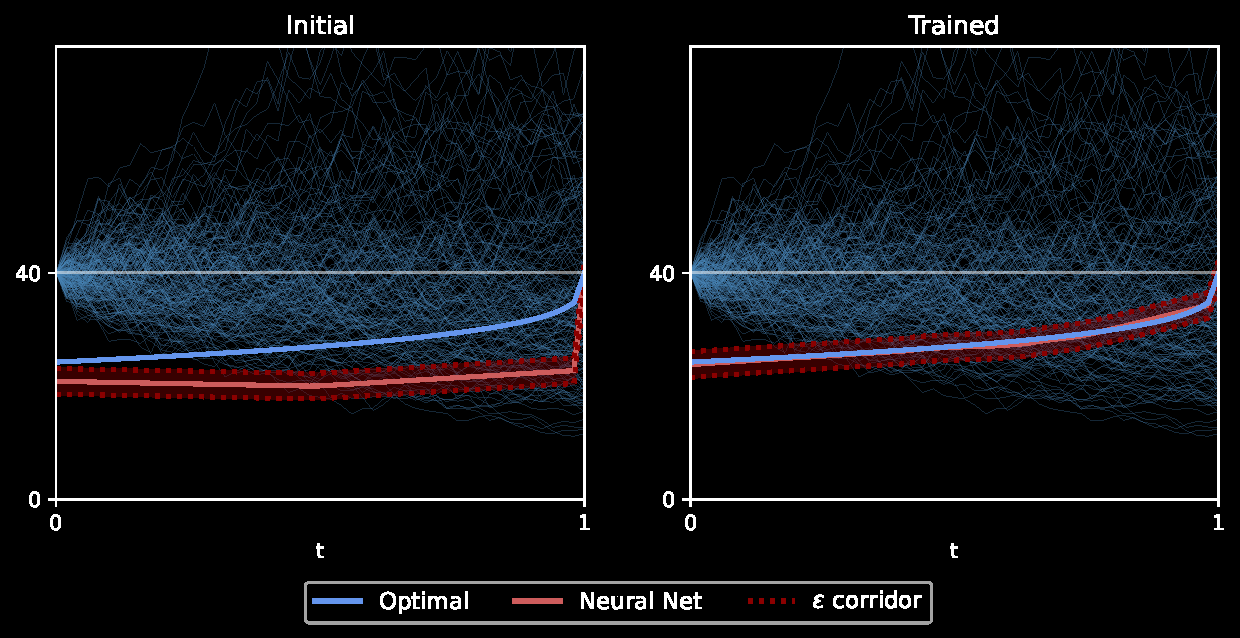
\includegraphics[scale=0.5]{Figures/Bdry 2, lbda=0.275, mu=0.050, N=50.pdf}
    
    \label{fig:putBS}
\end{figure}

\subsection{Put Option in the Heston Model}\label{sec:putHeston}

Consider the Bermudan put option from the previous section ($S_0 =K=40$, $T=1$, $N=50$) in the Heston model. Our goal is to see how stochastic volatility impacts the exercise boundary and  corresponding  price.   
 Let $m=1, \ k=0$ and assume the stock and factor dynamics
\begin{align*}
   \frac{dS_t}{S_t} &= (r-\delta)dt + \sqrt{\calV_t}\  dW_t, \\
   d\calV_t &= (\kappa(\bar{\nu}-\calV_t) - \gamma^{\Q}\calV_t)dt + \sigma_{\calV} \sqrt{\calV_t}\  d\tilde{W}_t, 
\end{align*}
with $\calV_0 = \nu_0 \in \R^2_+$ and $\frac{d\langle W, \tilde{W} \rangle_t}{dt} = \rho  \in  (-1,1)$. 
We choose the parameters
 $r = 6\%$, $\delta = 0\%$, $\kappa = 1$, $\nu_0 = \bar{\nu} = (40\%)^2$, $\gamma^{\Q} =0$, $\sigma_{\calV} =10\%$, and $\rho =-0.5$. In particular, 
the Feller condition $\kappa \,  \bar{\nu} \ge  \frac{\sigma_{\calV}^2}{2}$ is satisfied.  
For a fair comparison,  we set the initial value and long term mean of $\calV$ equal to the Black-Scholes variance $\sigma^2$ from \cref{sec:putBS}.   Moreover, we use importance sampling with same Girsanov parameter, i.e. $\lambda \equiv \frac{r-\delta + 0.05}{\sigma}  = 0.275$.

As seen in \cref{ex:vanilla}, the threshold function 
depends on time $t$ and the spot variance $\calV_t =\nu$.  
When $\varphi$ is convex and bounded (which is the case here)   \citet{LambertonHeston} showed that the value function $v(t,x)$, $x=(s,\nu)$, is  non-decreasing in $\nu$ for all $t\in [0,T]$. Consequently, the map $\nu \mapsto f(t,\nu)$ is non-increasing. As can be seen in  \cref{fig:heston1}, it turns out that the same holds for the trained neural network $G(\cdot,\cdot;\theta^M)$.
Notice also that $\nu \mapsto f(t,\nu)$ becomes less steep as $t$ approaches maturity. This is line with the fact that the Vega  decreases over time until the option is exercised.  
As $s \to v(t,s,\nu)$ is non-increasing for fixed $(t,\nu)$,  we therefore expect that the  rectangle $[0,s]\times [0,\nu]$ 
is contained in $\calS_t$ whenever $(s,\nu) \in \calS_t$. This is confirmed in  \cref{fig:heston1}. 

 \cref{tab:resultPutHeston} compares the price of the claim when the stopping decision exploit the spot variance ($f = f(t,\nu)$) and when it does not ($f = f(t)$). We observe that the price obtained with the "blind" strategy is significantly lower. Interestingly, the neural network coincides with the optimal boundary in the Black-Scholes model. %, as shown in Figure \cref{fig:heston1}
 Finally, \cref{fig:heston2} displays a trajectory for $(X,\calV)$ together with the threshold process $G(\cdot,\calV;\theta^M)$. As can be seen, the threshold is typically below the Black-Scholes boundary when $\calV_t$ is above its mean $\bar{\nu} = 0.16$ and vice versa. 

\begin{table}[ht]
  \centering
  \caption{Price of a Bermudan Put Option in the Heston model. \bb{(std to be reduced)}  
 }
  \begin{tabular}{c c c c }
 \hline  \hline
  Threshold function &  Price&  Std& Runtime  \\
  \hline  \hline
    $f(t,\nu)$ & 5.295 & 0.005 &  57.5 \\
  $f(t)$ & 5.281 & 0.006 &  57.5  \\
  \hline
\end{tabular}
\vspace{2mm}

\scriptsize{
\textit{Notes: The second and third column show the average and standard deviation of ten experiments, respectively.  }}
\label{tab:resultPutHeston}
  \end{table}
  
\begin{figure}[t]
    \centering
     \caption{Stopping and continuation regions (Bermudan put, Heston model).}
    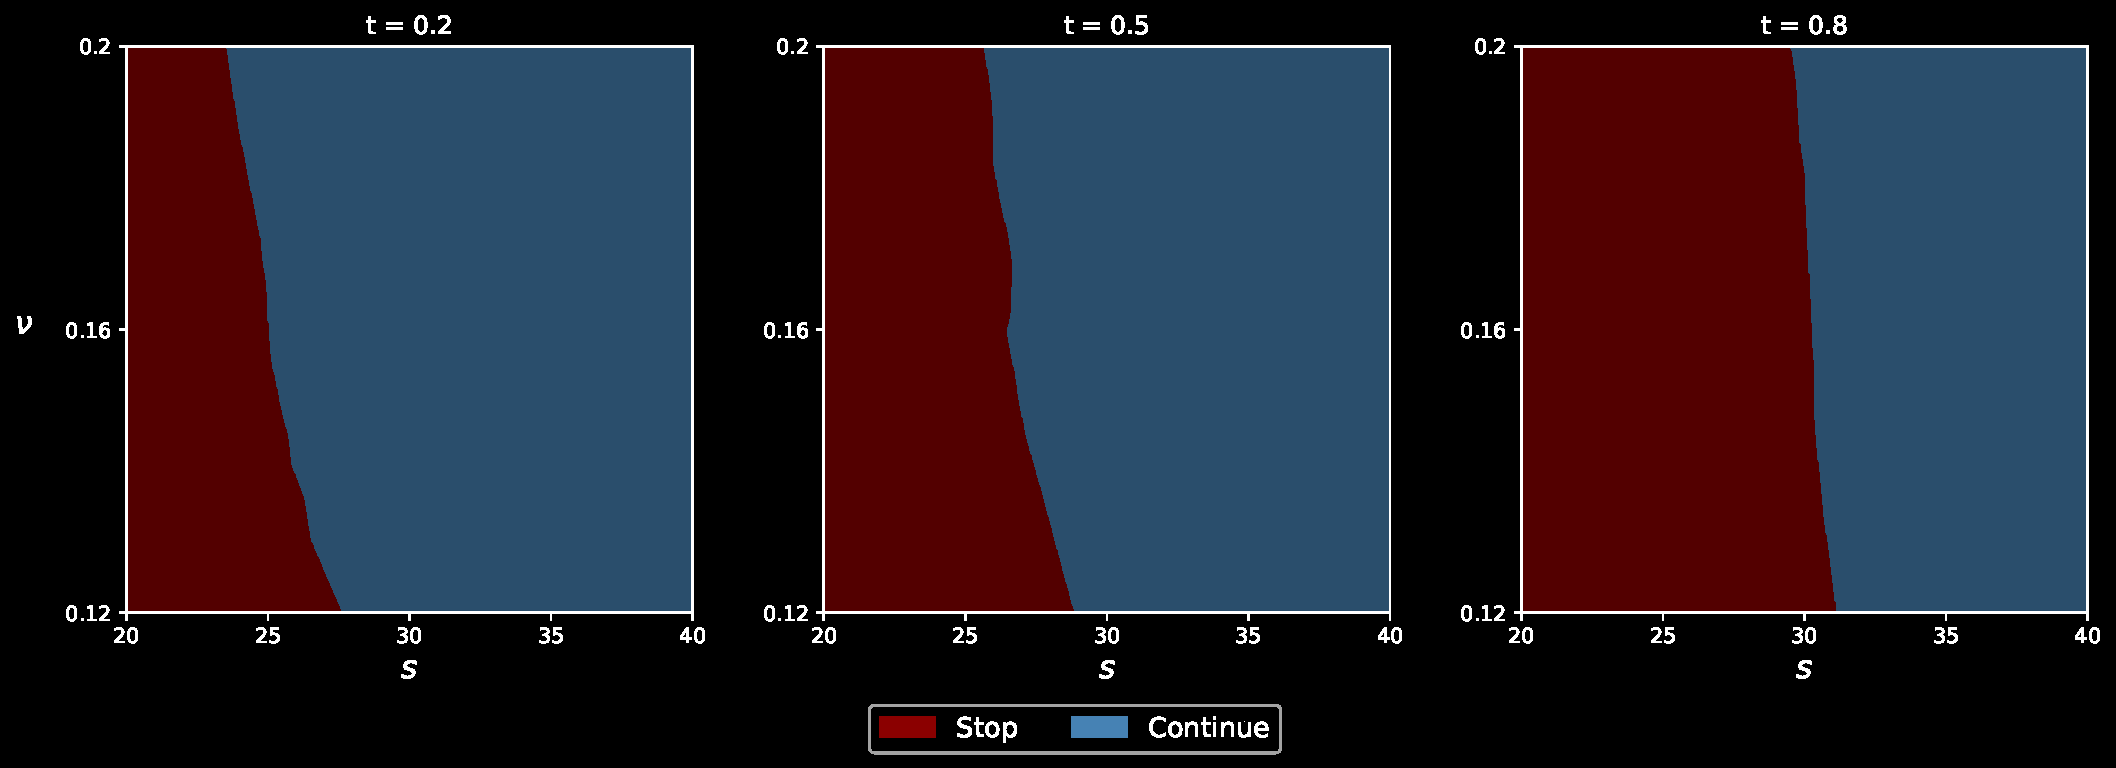
\includegraphics[scale = 0.42]{Figures/2DPlotHestonWide.pdf}
    \label{fig:heston1}
\end{figure}


\begin{figure}[t]
    \centering
     \caption{Stock price, variance and threshold process (Bermudan put, Heston model).}
    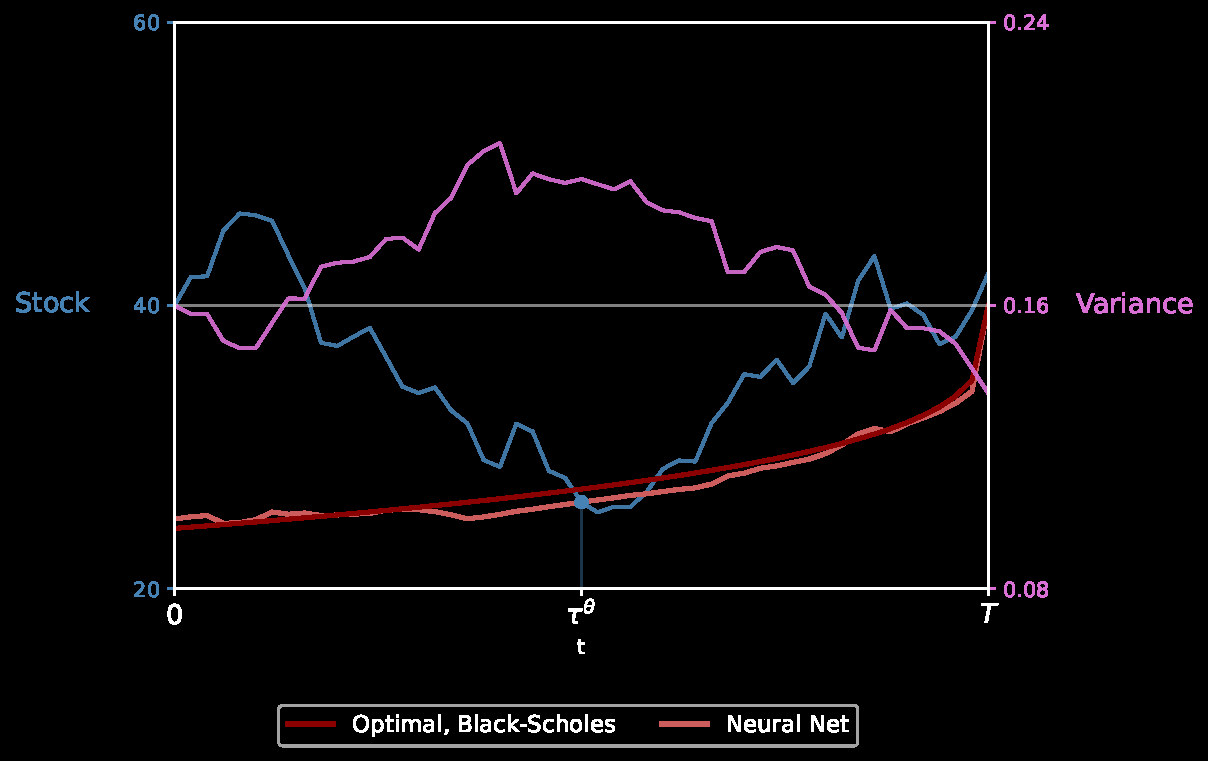
\includegraphics[scale = 0.42]{Figures/BdryHeston2.pdf}
    \label{fig:heston2}
\end{figure}


\subsection{High-dimensional Max Option on Symmetric Assets}\label{sec:maxCallSym}
Let $\alpha(s) = \max_{i=1,...,d}s_i$, $\beta\equiv 0$, $\eta=1$ and consider the multi-dimensional Black-Scholes model with independent and symmetric assets, i.e. 
\begin{align}\label{eq:BSAsym}
    d S_t = \text{diag}(S_t) \left[ (r\mathds{1} - \delta)dt + \sigma dW_t\right],
\end{align}
where $W$ is Brownian motion in $\R^d$, $r \in \R ,\sigma > 0$ and $\delta \in \R_+^d$. We employ the parameters from Section 4.4.1 in \cite{Becker2}, which are $s_0 =100 $, $r=5\%$, $\delta =10\%$ and $\sigma = 20 \%$. 

As both the payoff and assets are symmetric, it is easily shown that  $\calS_t$ is symmetric as well; see \cref{sec:symmetry}. This property can be exploited to reduce the dimension of our problem. Indeed, observe that it suffices to characterize the $t-$sections of the stopping region in the \textit{cone of ordered stocks}  
 $\calO = \{s\in \R_+^d \,|\, s_1 \geq \ldots \geq s_d\}$. We can therefore arrange $\Xi(S_t) = \frac{S_t}{\alpha(S_t)}\in [0,1]^d$ in decreasing order and give the outcome to $G(t,\cdot; \theta)$. If $\bar{S}_t \in \calO$ denotes the ordered version of $S_t$, then the last component of $\bar{S}_t$ are of little relevance to our stopping decision. 
 Indeed, over a short horizon, the maximum is  likely to be attained by the current best performing assets. %a stock having a high value today. 
 We can therefore set a cutoff $2 \le d' \ll d$ and feed the neural network with $(\frac{\bar{S}_{t,2}}{\alpha(S_t)},\ldots,\frac{\bar{S}_{t,d'}}{\alpha(S_t)})$ only.\footnote{Note that $\frac{\bar{S}_{t,1}}{\alpha(S_t)} \equiv 1$ is also removed from the neural network input as it doesn't carry any information.} Although one still needs to simulate $d$ assets, the size of the neural network can be significantly reduced, which in turn accelerates the training phase.  
 
 We illustrate this argument with $d=20$ assets and a cutoff of $d'=5$. 



\begin{table}[ht]
\caption{Max Option on $d \in\{5,10,20,50\}$ symmetric assetes}
\label{lab:symMaxOpt}
  \centering
  \begin{tabular}{ c c c c c c}
 \hline  \hline
   $d$ &  {\bf{Price}}&  {\bf{Std}}&  {\bf{Price in \cite{Becker2}}}&
    {\bf{Max Price}} & {\bf{Its Std}}\\
  \hline \hline
  5   & 26.1295 &  0.0095 & 26.147 &26.1506 &  0.0094 \\
 %\hline
  10   & 38.2735 &  0.0538 & 38.272 & 38.3351 &  0.0089  \\
    20   &  &   & 51.572 &  &    \\
 %\hline
  50  &  &   & 69.572  &  &   \\
 \hline
\end{tabular}

\vspace{2mm
}
 \scriptsize{
\textit{Notes: The second and third column show the average and standard deviation of ten experiments, respectively.  }}
  \end{table}
  
\subsection{Max Option on $d=2$ Asymmetric Assets}\label{sec:maxCallAsym}
Consider the multi-dimensional Black-Scholes model, i.e. 
\begin{align}\label{eq:BSAsym}
    d S_t = \text{diag}(S_t) \left[ (r\mathds{1} - \delta)dt + \sigma dW_t\right],
\end{align}
where $W$ is Brownian motion in $\R^d$, $r \in \R ,\sigma > 0$ and $\delta \in \R_+^d$. 
Define the connected components $\calS^{(i)}_t = \calS_t \cap \{\alpha(s) = s_i\}$, $i=1,2$ and the involution   $\varsigma(s_1,s_2) := (s_2,s_1)$.  

\begin{proposition} Consider a max option on $d=2$ assets with $S$ having dynamics as in $\eqref{eq:BSAsym}$. If $\delta_1 \le \delta_2$, then $\varsigma(\calS^{(1)}_t) \subseteq \calS^{(2)}_t$. \rr{(to be verified numerically...)}
\end{proposition}

\begin{proof} (\bb{attempts...})
Let $t\in [0,T)$ and take any $\tau \in \calT_t$. Then, defining the event $B = \{S^{t,s_1}_{\tau,1} \ge  S^{t,s_2}_{\tau,2}\}$, this gives
\begin{align*}
    \E^{\Q}[D_{t,\tau} \varphi(S^{t,s}_{\tau}) ] &= \E^{\Q}[D_{t,\tau} (S^{t,s_1}_{\tau,1}-K)^+ \ \mathds{1}_{B} ] + \E^{\Q}[D_{t,\tau} (S^{t,s_2}_{\tau,2}-K)^+ \ \mathds{1}_{B^c} ]. 
\end{align*}
Since $\gamma := e^{(\delta_1-\delta_2)(\tau-t)} \le 1$, then  $\{\gamma S^{t,s_1}_{\tau,1} \ge  \gamma^{-1} S^{t,s_2}_{\tau,2}\} \subseteq B$. Moreover, note that $(\gamma S^{t,s_1}_{\tau,1},\gamma^{-1} S^{t,s_2}_{\tau,2}) \overset{d}{=} \varsigma(S^{t,\varsigma(s)}_{\tau})$. 
\begin{equation*}
    \E^{\Q}[D_{t,\tau} (S^{t,s_1}_{\tau,1}-K)^+ \ \mathds{1}_{B} ] \ge  \E^{\Q}\left[D_{t,\tau} (\gamma S^{t,s_1}_{\tau,1}-K)^+ \ \mathds{1}_{\{\gamma S^{t,s_1}_{\tau,1} \ge  \gamma^{-1} S^{t,s_2}_{\tau,2}\}} \right ] = \E^{\Q}[D_{t,\tau} ( S^{t,s_1}_{\tau,2}-K)^+ \ \mathds{1}_{B'} ],
\end{equation*}
with $B':= \{ S^{t,s_1}_{\tau,2} \ge  S^{t,s_2}_{\tau,1}\}$. On the other hand, note that $S^{t,s_2}_{\tau,2} \ge S^{t,s_1}_{\tau,1} \ge S^{t,s_2}_{\tau,1} $ on $B^c$. Hence, 
\begin{align*}
    \E^{\Q}[D_{t,\tau} (S^{t,s_2}_{\tau,2}-K)^+ \ \mathds{1}_{B^c} ] &\ge  \E^{\Q}[D_{t,\tau} (S^{t,s_2}_{\tau,1}-K)^+ \ \mathds{1}_{B^c} ]\\
    &\rr{\ge} \E^{\Q}[D_{t,\tau} (S^{t,s_2}_{\tau,1}-K)^+ \ \mathds{1}_{(B')^c} ].
\end{align*}
But $B^c \subseteq B$!

We would conclude: 
\begin{align*}
    \E^{\Q}[D_{t,\tau} \varphi(S^{t,s}_{\tau}) ] &\ge \E^{\Q}[D_{t,\tau} ( S^{t,s_1}_{\tau,2}-K)^+ \ \mathds{1}_{B'} ] + \E^{\Q}[D_{t,\tau} (S^{t,s_2}_{\tau,1}-K)^+ \ \mathds{1}_{(B')^c} ]\\ 
    &= \E^{\Q}[D_{t,\tau} \varphi(S^{t,\varsigma(s)}_{\tau}) ]. 
\end{align*}

...

To show: 
$$\E^{\Q}[ \varphi(S^{t,s}_{u}) ] \ge \E^{\Q}[ \varphi(S^{t,\varsigma(s)}_{u}) ], \quad \forall \ u \in [t,T].  $$
And multiply by $D_{t,u}$. 

E.g., use stochastic dominance $\alpha(S^{t,s}_{u}) \succ \alpha(S^{t,\varsigma(s)}_{u})$. And therefore, if $\varphi = \psi \circ \alpha$ with $\psi(a) \to 0$ as $a\to \infty$
\begin{align*}
    \E^{\Q}[\varphi(S^{t,s}_{u}) ] &= \int_0^{\infty} \psi(a) d\Q(\alpha(S^{t,s}_{u}) \le a) \\ 
    &=  - \int_0^{\infty} \Q(\alpha(S^{t,s}_{u}) \le a) d \psi(a) \\ 
    &\ge  - \int_0^{\infty} \Q(\alpha(S^{t,\varsigma(s)}_{u}) \le a) d \psi(a) \\ 
     &\ge  \E^{\Q}[\varphi(S^{t,\varsigma(s)}_{u}) ].
\end{align*}
 If needed,  use $\psi^N \uparrow \psi$  and the monotone convergence theorem.  
%$M^{t,s}_{u} \succ M^{t,\varsigma(s)}_{u} $, where $M^{t,s}_{u} = \alpha(S^{t,s}_{u})$. 
\end{proof}

\begin{figure}
    \centering
    \caption{Stopping and continuation regions (max option, $d=2$ assets, $T=3$).}
    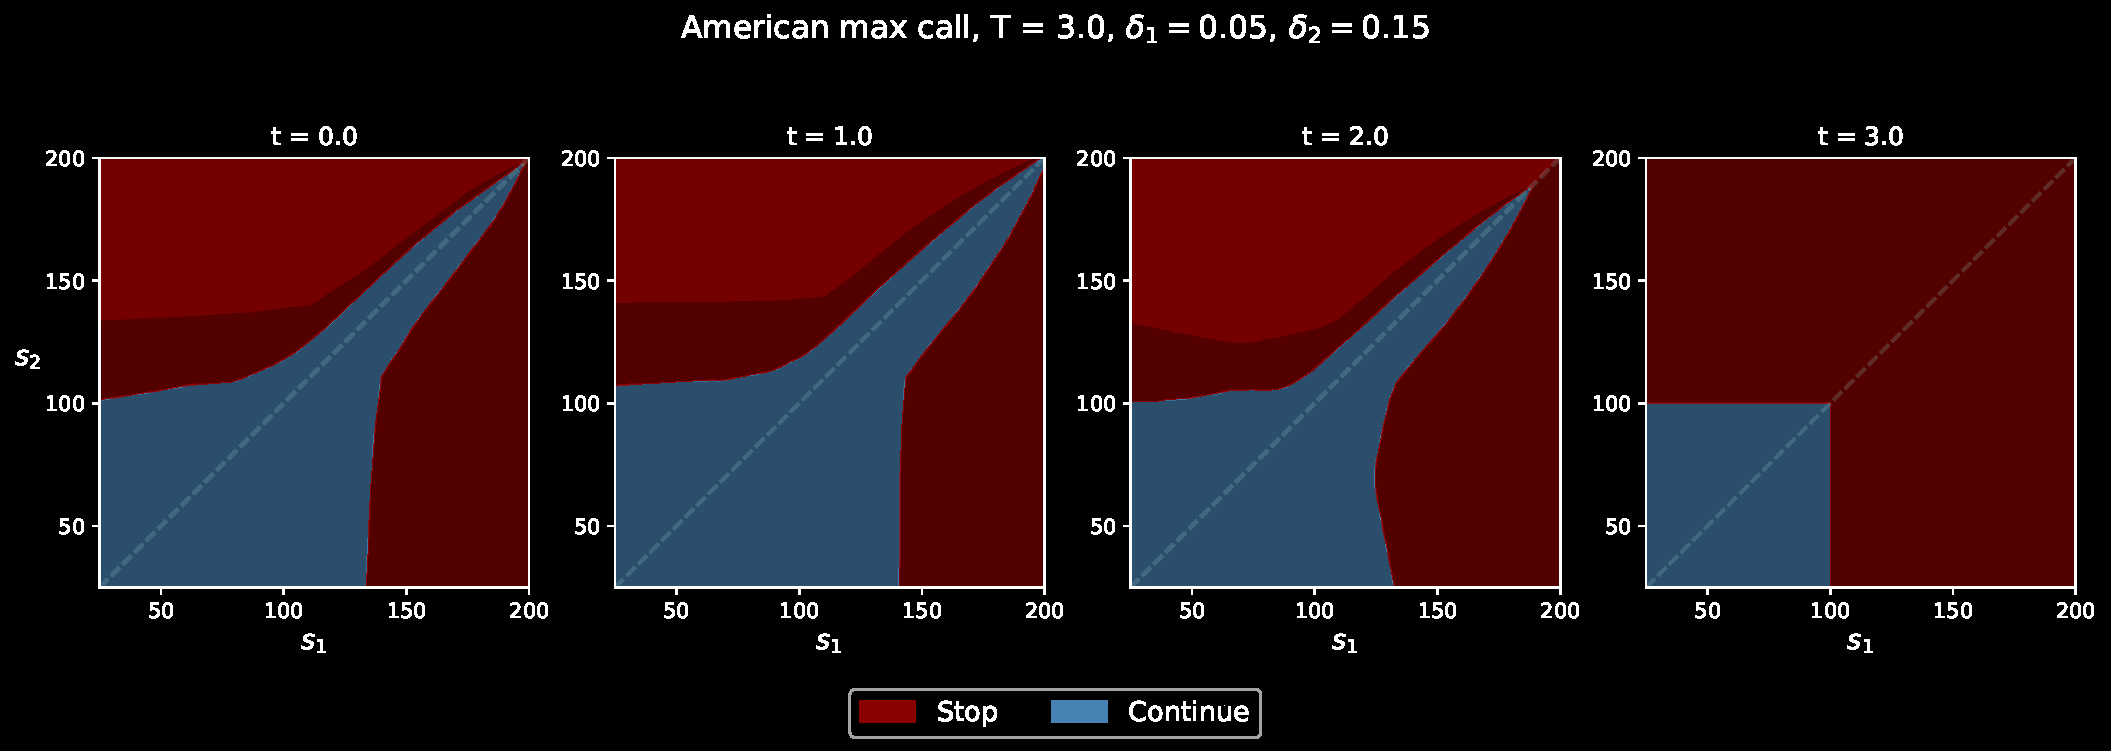
\includegraphics[scale = 0.42]{Figures/AsymMaxCall.pdf}
    \label{fig:asymCall}
    
    \scriptsize{
\textit{Notes: The light red region is the reflected image of $\calS_t^{(1)}$ through the diagonal, i.e. $\varsigma(\calS_t^{(1)})$.}} %This is to  illustrate that $\varsigma(\calS_t^{(1)}) \subseteq \calS_t^{(2)}$.  }}
\end{figure}

%\subsection{Spread Option}
%\subsection{Floating Strike Asian Option} \label{sec:Asian}
\subsection{Fixed Strike  Lookback Option} \label{sec:Lkbk}




%======= Conclusion ===========%
\section{Conclusion}  

\appendix 
% \setcounter{section}{0}
% \renewcommand*{\thesection}{\arabic{chapter}.\Alph{section}}

\section{Some Properties of the Stopping Region}
We briefly discuss some properties of the $t-$sections $\calS_t$ that are often relevant for the parametrization of the free boundary. 

\subsection{Symmetry}\label{sec:symmetry}

Many multi-asset, path-independent derivatives  present a type of symmetry in their payoff; see  \cref{ex:bskt} and \ref{ex:max}. Under certain conditions, this will carry over to the  stopping region. 
We assume $X=S$ throughout and  first recall the definition of symmetric functions. 

\begin{definition}
  A  function $\varphi: \R_+^d \to \R$ is called  \textit{symmetric} if it is invariant under permutation of its argument. Put differently, it must satisfy
    $$\varphi \circ \varsigma = \varphi, \quad \forall \ \varsigma \in \calP_{\! d} :=  \{\varsigma: \R^d_+ \mapsto \R^d_+ \, |\, \{s'_1,\ldots,s'_d\}=\{s_1,\ldots,s_d\}, \ s' = \varsigma(s) \}.$$%\{\varsigma: \R^d_+ \mapsto \R^d_+ \, |\, \varsigma(s)=(s_{i_1},...,s_{i_d}), \{i_1,...,i_d\} = \{1,...,d\} \}
   %with the group of permutations  $\calP_{\! d} =  \{\varsigma: \R^d_+ \mapsto \R^d_+ \, |\, \varsigma(s)=(s_{i_1},...,s_{i_d}), \{i_1,...,i_d\} = \{1,...,d\} \}.$
    %where $\calP_{\! d}$ is the group of permutations, 
    %$$\calP_d = \{\varsigma: \R^d_+ \mapsto \R^d_+ \, |\, \varsigma(s)=(s_{i_1},...,s_{i_d}), \{i_1,...,i_d\} = \{1,...,d\} \}.$$
\end{definition}

We also make the following distributional assumption on the stock prices.

\begin{asm}\label{asm: id} For all $(t,s)\in [0,T]\times \R_+^d$, the law of the forward-starting process $S^{t,s}$  is invariant under permutation, that is
    \begin{equation}\label{eq:id}
        \varsigma(S^{t,s}) \circ \Q = S^{t,\varsigma(s)} \circ  \Q, \quad \forall \ \varsigma \in \calP_{\!d}.
    \end{equation}
    % \begin{equation}
    %     \Q \circ (S^{t,s})^{-1} \circ \varsigma^{-1}  = \Q \circ (S^{t,\varsigma(s)})^{-1},
    % \end{equation}

    %The stock prices are identically distributed when starting at the same point, i.e. 
    %$$ \sigma(S^{t,\mathds{1}})  \circ \Pb = S^{t,\mathds{1}}  \circ \Pb \quad \forall \,\sigma \in \calP_d.$$
\end{asm}

Note that when Assumption \ref{asm: id} fails to hold,  the stopping region is in general not symmetric, regardless of the symmetry of $\varphi$; see \cref{sec:maxCallAsym}. 
The following result is now immediate.
\begin{proposition}
\label{prop:sym} Let $\varphi$
 be a symmetric payoff. If Assumption \ref{asm: id} holds, then the $t-$sections of the stopping region associated to $\varphi$ satisfy
$\varsigma(\calS_t)= \calS_t$ whatever $ \varsigma \in \calP_{\!d}$.
\end{proposition}
\begin{proof} Fix $t \in [0,T]$ and an arbitrary permutation $\varsigma \in \calP_d$. As $\varphi$ is symmetric, we show equivalently that $v(t,\cdot) \circ \varsigma =v(t,\cdot)$ with $v$ the associated value function. 
Given $\tau \in \calT_{\!t}$, we have
\begin{align*}\label{eq:proofSym}
    \E^{\Q}[\varphi(\tau,S^{t,s}_\tau)] =  \E^{\Q}[\varphi(\tau,\varsigma(S^{t,s}_\tau))] \
    \overset{\eqref{eq:id}}{=} \ \E^{\Q}[\varphi(\tau,S^{t,\varsigma(s)}_\tau)].
\end{align*}
Taking the supremum over all stopping times %on both sides %of $\eqref{eq:proofSym}$ 
yields the claim.
\end{proof}
Under the hypotheses of Proposition \ref{prop:sym}, it is sufficient to characterize the $t-$sections,  
$$\calV_t= \calS_t \cap \calO, \quad t \in [0,T], $$ where $\calO = \{s\in \R_+^d \,|\, s_1 \geq \ldots \geq s_d\}$ denotes the \textit{cone of ordered stocks}. The stopping region can be recovered by shuffling coordinates, namely $\calS_t = \bigcup_{\varsigma \in \calP_{\!d}} \varsigma(\calV_t)$ for $t\in[0,T]$.\footnote{Indeed, if $s\in  \bigcup_{\varsigma \in \calP_{\!d}} \varsigma(\calV_t)$, then $s=\varsigma(s')$ for some pair $(\varsigma,s') \in \calP_d \times \calV_t$. Hence 
$s \in \calS_t$ thanks to Proposition \ref{prop:sym}. Conversely for $s\in \calS_t$, there exists $\bar{\varsigma} \in \calP_d $ s.t. $s':=\bar{\varsigma}(s) \in \calO$ ($\bar{\varsigma}$ simply sorts  $s$ in non-increasing order). Proposition \ref{prop:sym} implies that $s' \in \calS_t$, which in turn gives   $ s' \in \calV_t$ and $s = \bar{\varsigma}^{\ -1}(s') \in \bigcup_{\varsigma \in \calP_d} \varsigma(\calV_t)$.} 
This fragmentation present benefits from a computational standpoint; see \cref{sec:maxCallSym}. 

 %Indeed, consider a max-call option on $d=2$ assets in the Black-Scholes model with same volatility but different dividend rates. Then \bb{...}
\subsubsection{Convexity}
Knowing topological properties of the unknown stopping region can help to characterize it more efficiently. We here focus on convexity. As the stopping region may not be connected (see \cref{ex:max}), we aim at determining when each connected component is convex.  We start off with some assumptions. 

\begin{asm}\label{asm:convlin}
$x \mapsto \varphi(x)$ is convex on $\calX$ and affine within each connected component of  $\calS_t$. 
\end{asm}

% Note that Assumption \ref{asm: convlin} is fulfilled by all payoffs from Section \ref{sec:examples}. Indeed, this is immediate when the functions $\alpha,  \beta$ in $\eqref{eq:payoff}$ are affine and for the max-option, the payoff is the positive part of a non-decreasing convex function, hence convex.   
We also need the following condition on $X$, which holds for instance for arithmetic and geometric Brownian motions. 
\begin{asm} \label{asm:affine}
    Given $0\le t \le u \le T$, the stochastic flow $x \mapsto X_u^{t,x}$  is an affine function.
\end{asm}

If both \cref{asm:scale} and  \ref{asm:affine}  hold, then necessarily $X_u^{t,x} = x \odot X_u^{t,\mathds{1}}$ so  the process is of "geometric" type. This leads us to the following result. 

\begin{proposition}
Under \cref{asm:convlin} and \ref{asm:affine}, $\calS_t$ is convex within each connected component.
\end{proposition}

\begin{proof}
Let $x,x'\in \calS_t$ belonging to the same connected component and  $\tilde{x}=\gamma x + (1-\gamma)x'$ for $\gamma \in [0,1]$. Then for all $\tau \in \calT_t$,
\begin{align*}
\E^{\Q}[D_{t,\tau}\varphi(X^{t,\tilde{x}}_\tau)] &=%\overset{\ref{asm:affine}}{=} 
\E^{\Q}[D_{t,\tau} \varphi(\gamma X^{t,x}_\tau + (1-\gamma) X^{t,x'}_\tau)]\\
    &\leq%\overset{\ref{asm:convlin}}{\leq}
    \gamma \E^{\Q}[D_{t,\tau}\varphi(X^{t,x}_\tau)]
    +
    (1-\gamma)\E^{\Q}[D_{t,\tau}\varphi(X^{t,x'}_\tau)]\\
    &\leq \gamma \varphi(x) + (1-\gamma) \varphi(x')\\
    &= %\overset{\ref{asm:convlin}}{=}
    \varphi(\tilde{x}).
\end{align*}
\end{proof}
Working with convex stopping regions is convenient as a continuum of stopping points can be deduced solely based on a few elements of $\calS_t$. Indeed, if we identify $x^{1},...,x^{J}$ as belonging to  $\calS_t$ %using the neural net $\Phi(\cdot;\theta)$,
, then   $\text{conv}(\{x^{1},...,x^{J}\}) \subseteq \calS_t$ as well.
\subsection{Monotonicity in Time}

\begin{proposition}\label{prop:monot}
Suppose that  $X$ and $D$ are stationary, that is $   
        X_u^{t,x} \circ \Q = X_{u-t}^{0,x} \circ  \Q \ $  and $D_{t,u} = D_{0,t-u}$ for every $t \le u $. 
Then the exercise boundary  expands over time, i.e. 
$ \calS_t \subseteq \calS_{t'}$ for all $t \le  t' $.

\end{proposition}
\begin{proof}
Take $t,t'\in [0,T]$ such that $\delta t := t'-t \ge 0$. %\footnote{The shift operator can be used, too.} 
 For  $\tau \in \calT_{t'}$, we have
\begin{align*}
    \E^{\Q}[D_{t',\tau}\varphi(X^{t',x}_{\tau})] &= \E^{\Q}[D_{t,\tau - \delta t }\varphi(X^{t,x}_{\tau - \delta t})] \le v(t,x), 
\end{align*}
as $\tau - \delta t \in \calT_t \cap \ [t,T-\delta t] \subseteq \calT_t$. If  $x\in \calS_t$, this gives   
$\E^{\Q}[D_{t',\tau}\varphi(X^{t',x}_{\tau})] \le  \varphi(x)$ for all $ \tau \in \calT_{t'} $ so  $x \in \calS_{t'}$ as claimed. 
\end{proof}

\begin{corollary}
\label{cor:monot} Let $f$ be the threshold function  as  in $\eqref{eq:thres}$. Then $t \mapsto f(t,\xi)$  is non-increasing for all $\xi \in \calE$.
\end{corollary}
\begin{proof}  Fix $\xi \in \calE$ and suppose that $a \in \calA_{t,\xi}$, i.e. $A^{-1}(a,\xi) \in \calS_t$. If $t' \ge t$, then $A^{-1}(a,\xi) \in \calS_{t'}$ as well from which we conclude that $\calA_{t,\xi} \subseteq \calA_{t',\xi}$. Thus $f(t',\xi) = \inf \calA_{t',\xi} \le \inf \calA_{t,\xi} = f(t,\xi)$. 
\end{proof}

% \begin{remark}
% If we  assume instead that the homeomorphism satisfies
% $$\left [ s\in \calS_t,\,  \Xi(s)=\Xi(s'), \,  \alpha(s')\geq \alpha(s) \right]  \Longrightarrow s'\in \calS_t,$$ (e.g. for a call-type payoff), then 
% $$f(t,x)= \inf \{a \in \R \, |\, A^{-1}(a,x) \in \calS_t\},$$
% and Corollary \ref{cor:monot} implies  that $t\mapsto f(t,x)$ is non-increasing.
% \end{remark}



Suppose that the payoff involves a parameter $K>0$, e.g. the strike of a vanilla option.  We write $\varphi_K$, $v_K$, $\calS_{t,K}$ and $f_K$ with the obvious notations. 
\begin{asm} \label{asm:homo}
The payoff is homogeneous in the sense that $\varphi_{K\gamma}(\gamma x)=\gamma \varphi_{K}(x)$, $\forall \  \gamma>0$. 
\end{asm}

\begin{proposition}\label{lem:homogen}
If  \cref{asm:scale} and \ref{asm:homo} hold,
then 
$\calS_{t,K}=K\calS_{t,1}:= \{Ks \,|\, s \in \calS_{t,1}\}.$
\end{proposition}
\begin{proof}
If $\varphi_K$ is homogeneous, then for all $t\in [0,T]$ and $\tau \in \calT_t$,
$$ \E[D_{t,\tau}\varphi_K(X^{t,x}_{\tau})] = \E[D_{t,\tau}\varphi_K(K X^{t,x/K}_{\tau})] =  K \E[D_{t,\tau} \varphi_1(X^{t,x/K}_{\tau})].$$
Thus $v_K(t,x) = K v(t,x/K)$, which finally gives 
\begin{align*}
    x \in \calS_{t,K} \Longleftrightarrow \varphi_K(x) = v_K(t,x)
    \Longleftrightarrow \varphi_1(x/K) = v_1(t,x/K)
    \Longleftrightarrow x \in K\calS_{t,1}.
\end{align*}
\end{proof}

% \begin{corollary}
% Suppose that the inverse function $A^{-1}: \R \times \calR \mapsto \R_+^d$ is homogeneous of degree $1$, i.e. $A^{-1}(a\gamma,x\gamma) = \gamma A^{-1}(a,x)$, $\gamma>0$. Then the exercise boundary satisfies
% $$f_K(t,x)= K \, f_1(t,x/K), \quad x \in \calR.$$
% \end{corollary}

% \begin{proof}
% Lemma \ref{lem:homogen} and the definition of $f_K$ directly give
% \begin{align*}
%     f_K(t,x) &= \sup \{a \in \R \,|\, A^{-1}(a,x) \in \calS_{t,K} \}\\
% &= \sup \{a \in \R \,|\, A^{-1}(a,x) \in K\calS_{t,1} \}\\
% &= \sup \left \{a \in \R \,|\, A^{-1}(a/K,x/K) \in \calS_{t,1}\right \}\\
% &= K f_1(t,x/K).
% \end{align*}

% \end{proof}

% \begin{example}
% Consider a basket
% option. A valid homeomorphism is  $A=(\alpha,\Xi)$ with  $$\alpha(s) = \frac{1}{d} \sum_{i=1}^d s_i, \quad \Xi(s) = s - \alpha(s).$$
% Then the inverse map $A^{-1}(a,x)=a+x$ is clearly homogeneous and the same therefore holds for $f_K$.
% \end{example}

% \begin{corollary}
% If the inverse map satisfies $A^{-1}(a\gamma,x) = \gamma A^{-1}(a,x)$, $\gamma>0$, then 
% $$f_K(t,x)= K \, f_1(t,x), \quad x \in \calR.$$
% \end{corollary}

% \begin{proof}
% Same argument as in the previous Corollary.
% \end{proof}

% \begin{example}
% For a max option, take $A=(\alpha,\Xi)$ with  $$\alpha(s) = s_1, \quad \Xi(s) = \frac{s}{s_1}.$$
% Then  $A^{-1}(a,x)=a x$ clearly verifies $A^{-1}(a\gamma,x) = \gamma A^{-1}(a,x)$ and thus $f_K(t,x)= K \, f_1(t,x) \; \forall  x \in \calR.$ Notice that this also holds for spread options.
% \end{example}

% \begin{corollary}
% The exercise boundary of American, single asset, vanilla options is homogeneous, i.e.
% $$f_K(t)= K \, f_1(t).$$
% \end{corollary}
% \begin{proof} It is clear that vanilla payoffs fulfill assumption \ref{asm:homo}.
% For  American puts, we get
% $$f_K(t) = \sup  \calS_{t,K} = \sup  K  \calS_{t,1} = K \sup \calS_{t,1} = K \, f_1(t).$$
% For  American calls, use infima instead.

%\renewcommand*{\thesection}{\arabic{chapter}.\arabic{section}}
%=============================%
\bibliography{refFB.bib}
%=============================%

\end{document}

